\documentclass{article}

\usepackage{../../noweb}
\noweboptions{smallcode,longchunks}

\usepackage[a4paper,margin=1in]{geometry}

\usepackage{colortbl}
\usepackage[colorlinks=true]{hyperref}
\usepackage{graphicx}

% Remove noweb page break penalty
\def\nwendcode{\endtrivlist \endgroup}
\let\nwdocspar=\par

\title{Jargo Storage Interface
  and Data Model\footnote{\url{https://github.com/jargors/Storage}}\\
  \vspace{.5em}
  \Large{\textbf{Correctness Test Program}}}
\author{James J. Pan\\
  \small{\href{mailto:jamesjpan@outlook.com}{jamesjpan@outlook.com}}
}

\begin{document}
\maketitle
\pagestyle{noweb}

\begin{figure}[h]
\centering
\fbox{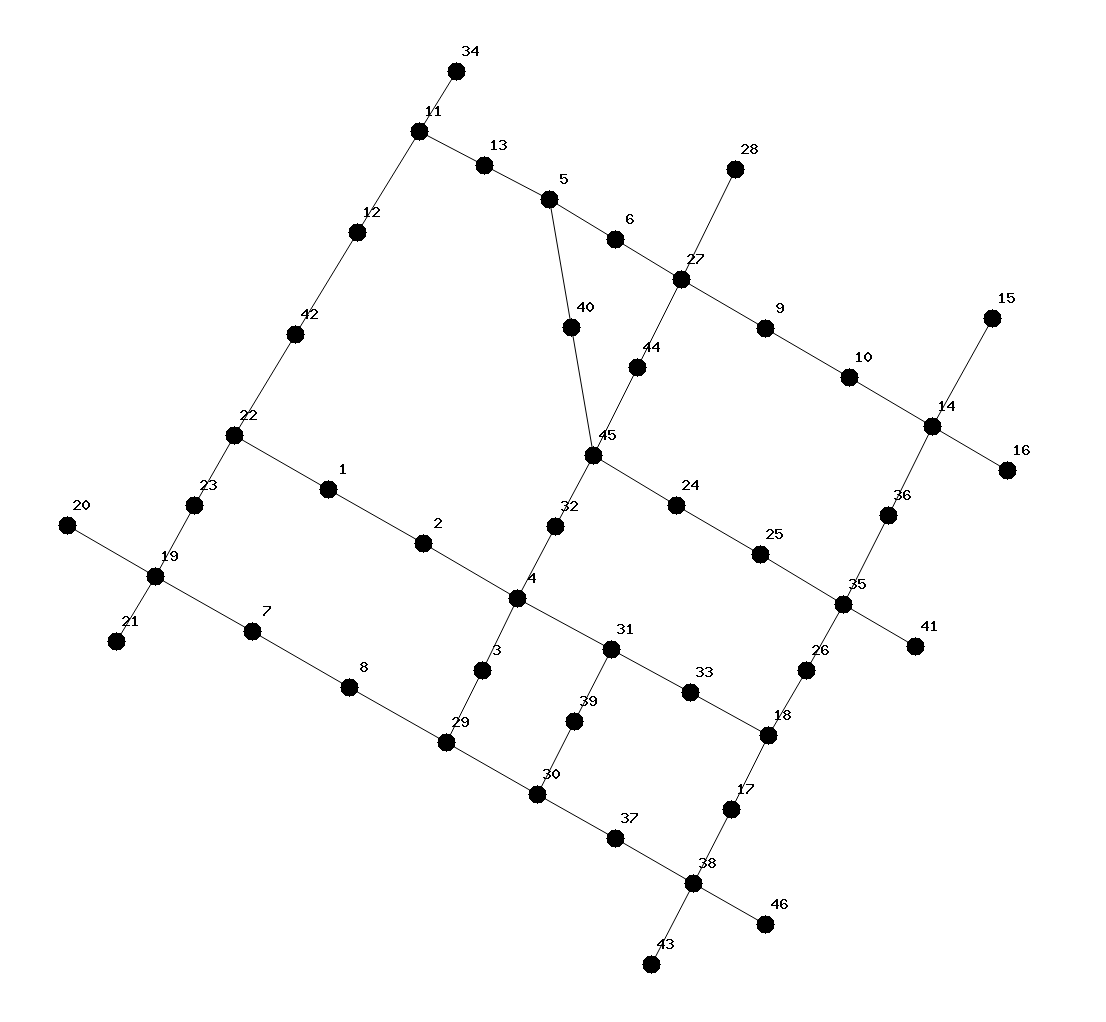
\includegraphics[width=\textwidth]{data/test.png}}
\caption{Portion of a road network in Chengdu, China,
    used for tests (46 nodes, 104 directed edges).}
\label{fig:road-network}
\end{figure}
\newpage

\tableofcontents

\section{Introduction}
\label{sec:introduction}
The correctness test program for Jargo's storage interface uses a series of
positive tests to check that the storage interface is functioning correctly.
These tests pass if the output from the storage interface matches with what is
expected. A database storing a test ridesharing state is provided in
{\tt{}data/db}.  The test road network is shown in Figure~\ref{fig:road-network}.
The vertex coordinates can be found in the Storage Test Generator program
({\tt{}generator/data/test.rnet}).  Beware, the tests are not comprehensive and do
not guarantee bug-free code. Not all possible inputs to the storage interface
methods are tested, although more comprehensive testing may be added in the
future.  The test program is developed using the
Noweb\footnote{\url{https://www.cs.tufts.edu/~nr/noweb/}} literate
programming\footnote{\url{http://literateprogramming.com/}} tool.  This file
({\tt{}src/StorageCorrectnessTest.nw}) is the source for both the documentation
({\tt{}doc/StorageCorrectnessTest.tex}) and the Java code
({\tt{}StorageCorrectnessTest.java})\footnote{See the {\tt{}Makefile} for build
details.}.
\nwfilename{src/StorageCorrectnessTest.nw}\nwbegincode{1}\sublabel{NW3KLP3H-SHxzk-1}\nwmargintag{{\nwtagstyle{}\subpageref{NW3KLP3H-SHxzk-1}}}\moddef{StorageCorrectnessTest.java~{\nwtagstyle{}\subpageref{NW3KLP3H-SHxzk-1}}}\endmoddef\nwnotused{StorageCorrectnessTest.java}
\LA{}StorageCorrectnessTest.java preamble~{\nwtagstyle{}\subpageref{NW3KLP3H-1P2gx-1}}\RA{}
\LA{}\code{}StorageCorrectnessTest\edoc{} definition~{\nwtagstyle{}\subpageref{NW3KLP3H-3wOKoY-1}}\RA{}
\nwendcode{}\nwbegindocs{2}\nwdocspar

\nwenddocs{}\nwbegincode{3}\sublabel{NW3KLP3H-1P2gx-1}\nwmargintag{{\nwtagstyle{}\subpageref{NW3KLP3H-1P2gx-1}}}\moddef{StorageCorrectnessTest.java preamble~{\nwtagstyle{}\subpageref{NW3KLP3H-1P2gx-1}}}\endmoddef\nwused{\\{NW3KLP3H-SHxzk-1}}
import com.github.jargors.Storage;
import com.github.jargors.Tools;
import com.github.jargors.exceptions.DuplicateVertexException;
import com.github.jargors.exceptions.DuplicateEdgeException;
import com.github.jargors.exceptions.DuplicateUserException;
import com.github.jargors.exceptions.EdgeNotFoundException;
import com.github.jargors.exceptions.UserNotFoundException;
import com.github.jargors.exceptions.VertexNotFoundException;
import java.time.LocalDateTime;
import java.sql.SQLException;
\nwendcode{}\nwbegindocs{4}\nwdocspar
\nwenddocs{}\nwbegincode{5}\sublabel{NW3KLP3H-3wOKoY-1}\nwmargintag{{\nwtagstyle{}\subpageref{NW3KLP3H-3wOKoY-1}}}\moddef{\code{}StorageCorrectnessTest\edoc{} definition~{\nwtagstyle{}\subpageref{NW3KLP3H-3wOKoY-1}}}\endmoddef\nwused{\\{NW3KLP3H-SHxzk-1}}
public class StorageCorrectnessTest \{
  \LA{}\code{}StorageCorrectnessTest\edoc{} member variables~{\nwtagstyle{}\subpageref{NW3KLP3H-e9ykQ-1}}\RA{}
  \LA{}\code{}StorageCorrectnessTest\edoc{} main routine~{\nwtagstyle{}\subpageref{NW3KLP3H-1EkuIK-1}}\RA{}
\}
\nwendcode{}\nwbegindocs{6}\nwdocspar
\nwenddocs{}\nwbegincode{7}\sublabel{NW3KLP3H-e9ykQ-1}\nwmargintag{{\nwtagstyle{}\subpageref{NW3KLP3H-e9ykQ-1}}}\moddef{\code{}StorageCorrectnessTest\edoc{} member variables~{\nwtagstyle{}\subpageref{NW3KLP3H-e9ykQ-1}}}\endmoddef\nwused{\\{NW3KLP3H-3wOKoY-1}}
private static int count_passed = 0;
private static int count_failed = 0;
\nwindexdefn{count{\char95}passed}{count:unpassed}{NW3KLP3H-e9ykQ-1}\nwindexdefn{count{\char95}failed}{count:unfailed}{NW3KLP3H-e9ykQ-1}\eatline
\nwidentdefs{\\{{count{\char95}failed}{count:unfailed}}\\{{count{\char95}passed}{count:unpassed}}}\nwendcode{}\nwbegincode{8}\sublabel{NW3KLP3H-1EkuIK-1}\nwmargintag{{\nwtagstyle{}\subpageref{NW3KLP3H-1EkuIK-1}}}\moddef{\code{}StorageCorrectnessTest\edoc{} main routine~{\nwtagstyle{}\subpageref{NW3KLP3H-1EkuIK-1}}}\endmoddef\nwused{\\{NW3KLP3H-3wOKoY-1}}
public static void main(String[] args) \{
  Storage storage = new Storage();
  Tools tools = new Tools();
  Tools.Print("Starting storage interface tests");
  try \{
    \LA{}Load test database~{\nwtagstyle{}\subpageref{NW3KLP3H-3tpa1X-1}}\RA{}
    \LA{}Run read tests~{\nwtagstyle{}\subpageref{NW3KLP3H-4Zn3Go-1}}\RA{}
    \LA{}Run write tests~{\nwtagstyle{}\subpageref{NW3KLP3H-3EijLo-1}}\RA{}
  \} catch (SQLException e) \{
    Tools.PrintSQLException(e);
  \} catch (Exception e) \{
    Tools.Print(e.toString());
  \}
  Tools.Print("Complete! Passed: "+count_passed+"; Failed: "+count_failed);
\}
\nwindexdefn{main}{main}{NW3KLP3H-1EkuIK-1}\eatline
\nwidentdefs{\\{{main}{main}}}\nwidentuses{\\{{count{\char95}failed}{count:unfailed}}\\{{count{\char95}passed}{count:unpassed}}}\nwindexuse{count{\char95}failed}{count:unfailed}{NW3KLP3H-1EkuIK-1}\nwindexuse{count{\char95}passed}{count:unpassed}{NW3KLP3H-1EkuIK-1}\nwendcode{}\nwbegindocs{9}We load a manually prepared test database.
\nwenddocs{}\nwbegincode{10}\sublabel{NW3KLP3H-3tpa1X-1}\nwmargintag{{\nwtagstyle{}\subpageref{NW3KLP3H-3tpa1X-1}}}\moddef{Load test database~{\nwtagstyle{}\subpageref{NW3KLP3H-3tpa1X-1}}}\endmoddef\nwused{\\{NW3KLP3H-1EkuIK-1}}
storage.DBLoadBackup("data/db");
storage.DBLoadRoadNetworkFromDB();
storage.DBLoadUsersFromDB();
\nwendcode{}\nwbegindocs{11}\nwdocspar
\section{Tests}
\label{sec:tests}

\subsection{Read Tests}
\label{sec:read-tests}
\nwenddocs{}\nwbegincode{12}\sublabel{NW3KLP3H-4Zn3Go-1}\nwmargintag{{\nwtagstyle{}\subpageref{NW3KLP3H-4Zn3Go-1}}}\moddef{Run read tests~{\nwtagstyle{}\subpageref{NW3KLP3H-4Zn3Go-1}}}\endmoddef\nwused{\\{NW3KLP3H-1EkuIK-1}}
\LA{}Test \code{}DBQuery\edoc{}(2)~{\nwtagstyle{}\subpageref{NW3KLP3H-49Fqm3-1}}\RA{}
\LA{}Test \code{}DBQueryServer\edoc{}(1)~{\nwtagstyle{}\subpageref{NW3KLP3H-3yzhzO-1}}\RA{}
\LA{}Test \code{}DBQueryRequest\edoc{}(1)~{\nwtagstyle{}\subpageref{NW3KLP3H-15uIOn-1}}\RA{}
\LA{}Test \code{}DBQueryQueuedRequests\edoc{}(1)~{\nwtagstyle{}\subpageref{NW3KLP3H-3kKW1I-1}}\RA{}
\LA{}Test \code{}DBQueryActiveServers\edoc{}(1)~{\nwtagstyle{}\subpageref{NW3KLP3H-1VRl4A-1}}\RA{}
\LA{}Test \code{}DBQueryServerLocationsAll\edoc{}(1)~{\nwtagstyle{}\subpageref{NW3KLP3H-2znKh3-1}}\RA{}
\LA{}Test \code{}DBQueryServerLocationsActive\edoc{}(1)~{\nwtagstyle{}\subpageref{NW3KLP3H-29RW2s-1}}\RA{}
\LA{}Test \code{}DBQueryServerRoute\edoc{}(1)~{\nwtagstyle{}\subpageref{NW3KLP3H-2ZTscP-1}}\RA{}
\LA{}Test \code{}DBQueryServerRemainingRoute\edoc{}(2)~{\nwtagstyle{}\subpageref{NW3KLP3H-2Xu2fm-1}}\RA{}
\LA{}Test \code{}DBQueryServerSchedule\edoc{}(1)~{\nwtagstyle{}\subpageref{NW3KLP3H-pl12h-1}}\RA{}
\LA{}Test \code{}DBQueryServerRemainingSchedule\edoc{}(2)~{\nwtagstyle{}\subpageref{NW3KLP3H-3OfygW-1}}\RA{}
\LA{}Test \code{}DBQueryServerMaxLoad\edoc{}(2)~{\nwtagstyle{}\subpageref{NW3KLP3H-2zdYPZ-1}}\RA{}
\LA{}Test \code{}DBQueryCountVertices\edoc{}(0)~{\nwtagstyle{}\subpageref{NW3KLP3H-2fQwdR-1}}\RA{}
\LA{}Test \code{}DBQueryCountEdges\edoc{}(0)~{\nwtagstyle{}\subpageref{NW3KLP3H-bumzO-1}}\RA{}
\LA{}Test \code{}DBQueryVertex\edoc{}(1)~{\nwtagstyle{}\subpageref{NW3KLP3H-22G5wj-1}}\RA{}
\LA{}Test \code{}DBQueryEdge\edoc{}(2)~{\nwtagstyle{}\subpageref{NW3KLP3H-3epPrx-1}}\RA{}
\LA{}Test \code{}DBQueryStatisticsEdges\edoc{}(0)~{\nwtagstyle{}\subpageref{NW3KLP3H-2uxshM-1}}\RA{}
\LA{}Test \code{}DBQueryMBR\edoc{}(0)~{\nwtagstyle{}\subpageref{NW3KLP3H-1n5ds2-1}}\RA{}
\LA{}Test \code{}DBQueryCountServers\edoc{}(0)~{\nwtagstyle{}\subpageref{NW3KLP3H-2F7I8K-1}}\RA{}
\LA{}Test \code{}DBQueryCountRequests\edoc{}(0)~{\nwtagstyle{}\subpageref{NW3KLP3H-rWzjn-1}}\RA{}
\LA{}Test \code{}DBQueryServerPendingAssignments\edoc{}(2)~{\nwtagstyle{}\subpageref{NW3KLP3H-2BxAR-1}}\RA{}
\LA{}Test \code{}DBQueryServerCompletedAssignments\edoc{}(2)~{\nwtagstyle{}\subpageref{NW3KLP3H-5lUDq-1}}\RA{}
\LA{}Test \code{}DBQueryServiceRate\edoc{}(0)~{\nwtagstyle{}\subpageref{NW3KLP3H-3be6sn-1}}\RA{}
\LA{}Test \code{}DBQueryBaseDistanceTotal\edoc{}(0)~{\nwtagstyle{}\subpageref{NW3KLP3H-NYCra-1}}\RA{}
\LA{}Test \code{}DBQueryServerBaseDistanceTotal\edoc{}(0)~{\nwtagstyle{}\subpageref{NW3KLP3H-4SurDP-1}}\RA{}
\LA{}Test \code{}DBQueryRequestBaseDistanceTotal\edoc{}(0)~{\nwtagstyle{}\subpageref{NW3KLP3H-2dPBT8-1}}\RA{}
\LA{}Test \code{}DBQueryServerTravelDistance\edoc{}(1)~{\nwtagstyle{}\subpageref{NW3KLP3H-nARGd-1}}\RA{}
\LA{}Test \code{}DBQueryServerTravelDistanceTotal\edoc{}(0)~{\nwtagstyle{}\subpageref{NW3KLP3H-TK2Pq-1}}\RA{}
\LA{}Test \code{}DBQueryServerCruisingDistance\edoc{}(1)~{\nwtagstyle{}\subpageref{NW3KLP3H-1lg9ot-1}}\RA{}
\LA{}Test \code{}DBQueryServerCruisingDistanceTotal\edoc{}(0)~{\nwtagstyle{}\subpageref{NW3KLP3H-3u3QCX-1}}\RA{}
\LA{}Test \code{}DBQueryServerServiceDistance\edoc{}(1)~{\nwtagstyle{}\subpageref{NW3KLP3H-2EvAhx-1}}\RA{}
\LA{}Test \code{}DBQueryServerServiceDistanceTotal\edoc{}(0)~{\nwtagstyle{}\subpageref{NW3KLP3H-3lRmMQ-1}}\RA{}
\LA{}Test \code{}DBQueryRequestDetourDistance\edoc{}(1)~{\nwtagstyle{}\subpageref{NW3KLP3H-4G59p1-1}}\RA{}
\LA{}Test \code{}DBQueryRequestDetourDistanceTotal\edoc{}(0)~{\nwtagstyle{}\subpageref{NW3KLP3H-iqssa-1}}\RA{}
\LA{}Test \code{}DBQueryRequestTransitDistance\edoc{}(1)~{\nwtagstyle{}\subpageref{NW3KLP3H-2jtv8e-1}}\RA{}
\LA{}Test \code{}DBQueryRequestTransitDistanceTotal\edoc{}(0)~{\nwtagstyle{}\subpageref{NW3KLP3H-2ceAow-1}}\RA{}
\LA{}Test \code{}DBQueryServerTravelDuration\edoc{}(1)~{\nwtagstyle{}\subpageref{NW3KLP3H-1ym97n-1}}\RA{}
\LA{}Test \code{}DBQueryServerTravelDurationTotal\edoc{}(0)~{\nwtagstyle{}\subpageref{NW3KLP3H-V1f4r-1}}\RA{}
\LA{}Test \code{}DBQueryRequestPickupDuration\edoc{}(1)~{\nwtagstyle{}\subpageref{NW3KLP3H-1u1Y5e-1}}\RA{}
\LA{}Test \code{}DBQueryRequestPickupDurationTotal\edoc{}(0)~{\nwtagstyle{}\subpageref{NW3KLP3H-1YcttO-1}}\RA{}
\LA{}Test \code{}DBQueryRequestTransitDuration\edoc{}(1)~{\nwtagstyle{}\subpageref{NW3KLP3H-3rLBYG-1}}\RA{}
\LA{}Test \code{}DBQueryRequestTransitDurationTotal\edoc{}(0)~{\nwtagstyle{}\subpageref{NW3KLP3H-2awpm1-1}}\RA{}
\LA{}Test \code{}DBQueryRequestTravelDuration\edoc{}(1)~{\nwtagstyle{}\subpageref{NW3KLP3H-l7awQ-1}}\RA{}
\LA{}Test \code{}DBQueryRequestTravelDurationTotal\edoc{}(0)~{\nwtagstyle{}\subpageref{NW3KLP3H-1MG8Jy-1}}\RA{}
\LA{}Test \code{}DBQueryRequestDepartureTime\edoc{}(1)~{\nwtagstyle{}\subpageref{NW3KLP3H-cK1ti-1}}\RA{}
\LA{}Test \code{}DBQueryServerDepartureTime\edoc{}(1)~{\nwtagstyle{}\subpageref{NW3KLP3H-2I5qzs-1}}\RA{}
\LA{}Test \code{}DBQueryRequestArrivalTime\edoc{}(1)~{\nwtagstyle{}\subpageref{NW3KLP3H-299kaf-1}}\RA{}
\LA{}Test \code{}DBQueryServerArrivalTime\edoc{}(1)~{\nwtagstyle{}\subpageref{NW3KLP3H-4RKxvl-1}}\RA{}
\nwendcode{}\nwbegindocs{13}\nwdocspar

\subsubsection{{\tt{}DBQuery}(2)}
Test {\tt{}DBQuery}(2) with a simple select statement. The road network has
46 vertices, plus 1 dummy vertex for a total of 47 vertices.
\nwenddocs{}\nwbegincode{14}\sublabel{NW3KLP3H-49Fqm3-1}\nwmargintag{{\nwtagstyle{}\subpageref{NW3KLP3H-49Fqm3-1}}}\moddef{Test \code{}DBQuery\edoc{}(2)~{\nwtagstyle{}\subpageref{NW3KLP3H-49Fqm3-1}}}\endmoddef\nwused{\\{NW3KLP3H-4Zn3Go-1}}
\{
  int output[] = storage.DBQuery("SELECT COUNT (*) FROM V", 1);
  if (output[0] != 47) \{
    Tools.Print("[FAIL] DBQuery(2)");
    Tools.Print("\\tExpected 47; got "+output[0]);
    count_failed++;
  \} else \{
    Tools.Print("[PASS] DBQuery(2)");
    count_passed++;
  \}
\}
\nwidentuses{\\{{count{\char95}failed}{count:unfailed}}\\{{count{\char95}passed}{count:unpassed}}}\nwindexuse{count{\char95}failed}{count:unfailed}{NW3KLP3H-49Fqm3-1}\nwindexuse{count{\char95}passed}{count:unpassed}{NW3KLP3H-49Fqm3-1}\nwendcode{}\nwbegindocs{15}\nwdocspar

\subsubsection{{\tt{}DBQueryServer}(1)}
\nwenddocs{}\nwbegincode{16}\sublabel{NW3KLP3H-3yzhzO-1}\nwmargintag{{\nwtagstyle{}\subpageref{NW3KLP3H-3yzhzO-1}}}\moddef{Test \code{}DBQueryServer\edoc{}(1)~{\nwtagstyle{}\subpageref{NW3KLP3H-3yzhzO-1}}}\endmoddef\nwused{\\{NW3KLP3H-4Zn3Go-1}}
\{
  int output[] = storage.DBQueryUser(1);
  if (!(output[0] == 1
     && output[1] == -10
     && output[2] == 1
     && output[3] == 500
     && output[4] == 22
     && output[5] == 0
     && output[6] == 0)) \{
    Tools.Print("[FAIL] DBQueryUser(1)");
    Tools.Print("\\tExpected \{uid=1, q=-10, e=1, l=500, o=22, d=0, b=0\}; got");
    tools.printUser(output);
    count_failed++;
  \} else \{
    Tools.Print("[PASS] DBQueryUser(1)");
    count_passed++;
  \}
\}
\nwidentuses{\\{{count{\char95}failed}{count:unfailed}}\\{{count{\char95}passed}{count:unpassed}}}\nwindexuse{count{\char95}failed}{count:unfailed}{NW3KLP3H-3yzhzO-1}\nwindexuse{count{\char95}passed}{count:unpassed}{NW3KLP3H-3yzhzO-1}\nwendcode{}\nwbegindocs{17}\nwdocspar
\subsubsection{{\tt{}DBQueryRequest}(1)}
\nwenddocs{}\nwbegincode{18}\sublabel{NW3KLP3H-15uIOn-1}\nwmargintag{{\nwtagstyle{}\subpageref{NW3KLP3H-15uIOn-1}}}\moddef{Test \code{}DBQueryRequest\edoc{}(1)~{\nwtagstyle{}\subpageref{NW3KLP3H-15uIOn-1}}}\endmoddef\nwused{\\{NW3KLP3H-4Zn3Go-1}}
\{
  int output[] = storage.DBQueryUser(10);
  if (!(output[0] == 10
     && output[1] == 1
     && output[2] == 0
     && output[3] == 500
     && output[4] == 4
     && output[5] == 30
     && output[6] == 172)) \{
    Tools.Print("[FAIL] DBQueryUser(1)");
    Tools.Print("\\tExpected \{uid=10, q=1, e=0, l=500, o=4, d=30, b=172\}; got");
    tools.printUser(output);
    count_failed++;
  \} else \{
    Tools.Print("[PASS] DBQueryUser(1)");
    count_passed++;
  \}
\}
\nwidentuses{\\{{count{\char95}failed}{count:unfailed}}\\{{count{\char95}passed}{count:unpassed}}}\nwindexuse{count{\char95}failed}{count:unfailed}{NW3KLP3H-15uIOn-1}\nwindexuse{count{\char95}passed}{count:unpassed}{NW3KLP3H-15uIOn-1}\nwendcode{}\nwbegindocs{19}\nwdocspar
\subsubsection{{\tt{}DBQueryQueuedRequests}(1)}
In the test database, Request 11 is never assigned. It appears
at $t=5$ and times out after $t=35$.
\nwenddocs{}\nwbegincode{20}\sublabel{NW3KLP3H-3kKW1I-1}\nwmargintag{{\nwtagstyle{}\subpageref{NW3KLP3H-3kKW1I-1}}}\moddef{Test \code{}DBQueryQueuedRequests\edoc{}(1)~{\nwtagstyle{}\subpageref{NW3KLP3H-3kKW1I-1}}}\endmoddef\nwused{\\{NW3KLP3H-4Zn3Go-1}}
\{
  \LA{}..test \code{}DBQueryQueuedRequests\edoc{}(1) at t=0~{\nwtagstyle{}\subpageref{NW3KLP3H-Zjogp-1}}\RA{}
  \LA{}..test \code{}DBQueryQueuedRequests\edoc{}(1) at t=5~{\nwtagstyle{}\subpageref{NW3KLP3H-3wMzIF-1}}\RA{}
  \LA{}..test \code{}DBQueryQueuedRequests\edoc{}(1) at t=35~{\nwtagstyle{}\subpageref{NW3KLP3H-1wCq8e-1}}\RA{}
  \LA{}..test \code{}DBQueryQueuedRequests\edoc{}(1) at t=36~{\nwtagstyle{}\subpageref{NW3KLP3H-4DZ4um-1}}\RA{}
\}
\nwendcode{}\nwbegindocs{21}\nwdocspar
As Request 11 has not appeared yet at $t=0$, we expect
{\tt{}DBQueryQueuedRequests} to return nothing.
\nwenddocs{}\nwbegincode{22}\sublabel{NW3KLP3H-Zjogp-1}\nwmargintag{{\nwtagstyle{}\subpageref{NW3KLP3H-Zjogp-1}}}\moddef{..test \code{}DBQueryQueuedRequests\edoc{}(1) at t=0~{\nwtagstyle{}\subpageref{NW3KLP3H-Zjogp-1}}}\endmoddef\nwused{\\{NW3KLP3H-3kKW1I-1}}
\{
  int output[] = storage.DBQueryQueuedRequests(0);
  if (!(output.length/7 == 0)) \{
    Tools.Print("[FAIL] DBQueryQueuedRequests(1) (1/4)");
    Tools.Print("\\tExpected 0; got "+output.length/7);
    count_failed++;
  \} else \{
    Tools.Print("[PASS] DBQueryQueuedRequests(1) (1/4)");
    count_passed++;
  \}
\}
\nwidentuses{\\{{count{\char95}failed}{count:unfailed}}\\{{count{\char95}passed}{count:unpassed}}}\nwindexuse{count{\char95}failed}{count:unfailed}{NW3KLP3H-Zjogp-1}\nwindexuse{count{\char95}passed}{count:unpassed}{NW3KLP3H-Zjogp-1}\nwendcode{}\nwbegindocs{23}\nwdocspar
At $t=5$, Request 11 should have just appeared and be queued up.
\nwenddocs{}\nwbegincode{24}\sublabel{NW3KLP3H-3wMzIF-1}\nwmargintag{{\nwtagstyle{}\subpageref{NW3KLP3H-3wMzIF-1}}}\moddef{..test \code{}DBQueryQueuedRequests\edoc{}(1) at t=5~{\nwtagstyle{}\subpageref{NW3KLP3H-3wMzIF-1}}}\endmoddef\nwused{\\{NW3KLP3H-3kKW1I-1}}
\{
  int output[] = storage.DBQueryQueuedRequests(5);
  if (!(output.length/7 == 1)) \{
    Tools.Print("[FAIL] DBQueryQueuedRequests(1) (2/4)");
    Tools.Print("\\tExpected 1; got "+output.length/7);
    count_failed++;
  \} else if (!(output[0] == 11)
    && (output[1] == 1)
    && (output[2] == 5)
    && (output[3] == 500)
    && (output[4] == 1)
    && (output[5] == 32)
    && (output[6] == 194)) \{
    Tools.Print("[FAIL] DBQueryQueuedRequests(1) (2/4)");
    Tools.Print("\\tExpected \{uid=11, q=1, e=5, l=500, o=1, d=32, b=194\}; got");
    tools.printUser(output);
    count_failed++;
  \} else \{
    Tools.Print("[PASS] DBQueryQueuedRequests(1) (2/4)");
    count_passed++;
  \}
\}
\nwidentuses{\\{{count{\char95}failed}{count:unfailed}}\\{{count{\char95}passed}{count:unpassed}}}\nwindexuse{count{\char95}failed}{count:unfailed}{NW3KLP3H-3wMzIF-1}\nwindexuse{count{\char95}passed}{count:unpassed}{NW3KLP3H-3wMzIF-1}\nwendcode{}\nwbegindocs{25}\nwdocspar
At $t=35$, Request 11 should be just about to time out but still in the queue.
\nwenddocs{}\nwbegincode{26}\sublabel{NW3KLP3H-1wCq8e-1}\nwmargintag{{\nwtagstyle{}\subpageref{NW3KLP3H-1wCq8e-1}}}\moddef{..test \code{}DBQueryQueuedRequests\edoc{}(1) at t=35~{\nwtagstyle{}\subpageref{NW3KLP3H-1wCq8e-1}}}\endmoddef\nwused{\\{NW3KLP3H-3kKW1I-1}}
\{
  int output[] = storage.DBQueryQueuedRequests(35);
  if (!(output.length/7 == 1)) \{
    Tools.Print("[FAIL] DBQueryQueuedRequests(1) (3/4)");
    Tools.Print("\\tExpected 1; got "+output.length/7);
    count_failed++;
  \} else if (!(output[0] == 11)
    && (output[1] == 1)
    && (output[2] == 5)
    && (output[3] == 500)
    && (output[4] == 1)
    && (output[5] == 32)
    && (output[6] == 194)) \{
    Tools.Print("[FAIL] DBQueryQueuedRequests(1) (3/4)");
    Tools.Print("\\tExpected \{uid=11, q=1, e=5, l=500, o=1, d=32, b=194\}; got");
    tools.printUser(output);
    count_failed++;
  \} else \{
    Tools.Print("[PASS] DBQueryQueuedRequests(1) (3/4)");
    count_passed++;
  \}
\}
\nwidentuses{\\{{count{\char95}failed}{count:unfailed}}\\{{count{\char95}passed}{count:unpassed}}}\nwindexuse{count{\char95}failed}{count:unfailed}{NW3KLP3H-1wCq8e-1}\nwindexuse{count{\char95}passed}{count:unpassed}{NW3KLP3H-1wCq8e-1}\nwendcode{}\nwbegindocs{27}\nwdocspar
At $t>35$, Request 11 should be timed out and there should be no queued
requests.
\nwenddocs{}\nwbegincode{28}\sublabel{NW3KLP3H-4DZ4um-1}\nwmargintag{{\nwtagstyle{}\subpageref{NW3KLP3H-4DZ4um-1}}}\moddef{..test \code{}DBQueryQueuedRequests\edoc{}(1) at t=36~{\nwtagstyle{}\subpageref{NW3KLP3H-4DZ4um-1}}}\endmoddef\nwused{\\{NW3KLP3H-3kKW1I-1}}
\{
  int output[] = storage.DBQueryQueuedRequests(36);
  if (!(output.length/7 == 0)) \{
    Tools.Print("[FAIL] DBQueryQueuedRequests(1) (4/4)");
    Tools.Print("\\tExpected 0; got "+output.length/7);
    count_failed++;
  \} else \{
    Tools.Print("[PASS] DBQueryQueuedRequests(1) (4/4)");
    count_passed++;
  \}
\}
\nwidentuses{\\{{count{\char95}failed}{count:unfailed}}\\{{count{\char95}passed}{count:unpassed}}}\nwindexuse{count{\char95}failed}{count:unfailed}{NW3KLP3H-4DZ4um-1}\nwindexuse{count{\char95}passed}{count:unpassed}{NW3KLP3H-4DZ4um-1}\nwendcode{}\nwbegindocs{29}\nwdocspar

\subsubsection{{\tt{}DBQueryActiveServers}(1)}
We focus on four cases. When $t=0$, neither service has begun service yet,
and we expect no locations to be returned. When $t=44$, Server 2 is out of
service, and Server 1 has just arrived at vertex 30. When $t=45$, Server 1
has just ended service. When $t=46$, both Server 1 and Server 2 are out of
service.
\nwenddocs{}\nwbegincode{30}\sublabel{NW3KLP3H-1VRl4A-1}\nwmargintag{{\nwtagstyle{}\subpageref{NW3KLP3H-1VRl4A-1}}}\moddef{Test \code{}DBQueryActiveServers\edoc{}(1)~{\nwtagstyle{}\subpageref{NW3KLP3H-1VRl4A-1}}}\endmoddef\nwused{\\{NW3KLP3H-4Zn3Go-1}}
\{
  \LA{}..test \code{}DBQueryActiveServers\edoc{}(1) when $t=0$~{\nwtagstyle{}\subpageref{NW3KLP3H-YOSd5-1}}\RA{}
  \LA{}..test \code{}DBQueryActiveServers\edoc{}(1) when $t=44$~{\nwtagstyle{}\subpageref{NW3KLP3H-2YsBYF-1}}\RA{}
  \LA{}..test \code{}DBQueryActiveServers\edoc{}(1) when $t=45$~{\nwtagstyle{}\subpageref{NW3KLP3H-2Xvc8N-1}}\RA{}
  \LA{}..test \code{}DBQueryActiveServers\edoc{}(1) when $t=46$~{\nwtagstyle{}\subpageref{NW3KLP3H-2YUfrz-1}}\RA{}
\}
\nwendcode{}\nwbegindocs{31}\nwdocspar
\nwenddocs{}\nwbegincode{32}\sublabel{NW3KLP3H-YOSd5-1}\nwmargintag{{\nwtagstyle{}\subpageref{NW3KLP3H-YOSd5-1}}}\moddef{..test \code{}DBQueryActiveServers\edoc{}(1) when $t=0$~{\nwtagstyle{}\subpageref{NW3KLP3H-YOSd5-1}}}\endmoddef\nwused{\\{NW3KLP3H-1VRl4A-1}}
\{
  int output[] = storage.DBQueryActiveServers(0);
  if (!(output.length == 0)) \{
    Tools.Print("[FAIL] DBQueryActiveServers(1) (1/4)");
    Tools.Print("\\tExpected 0; got "+output.length/3);
    count_failed++;
  \} else \{
    Tools.Print("[PASS] DBQueryActiveServers(1) (1/4)");
    count_passed++;
  \}
\}
\nwidentuses{\\{{count{\char95}failed}{count:unfailed}}\\{{count{\char95}passed}{count:unpassed}}}\nwindexuse{count{\char95}failed}{count:unfailed}{NW3KLP3H-YOSd5-1}\nwindexuse{count{\char95}passed}{count:unpassed}{NW3KLP3H-YOSd5-1}\nwendcode{}\nwbegindocs{33}\nwdocspar
\nwenddocs{}\nwbegincode{34}\sublabel{NW3KLP3H-2YsBYF-1}\nwmargintag{{\nwtagstyle{}\subpageref{NW3KLP3H-2YsBYF-1}}}\moddef{..test \code{}DBQueryActiveServers\edoc{}(1) when $t=44$~{\nwtagstyle{}\subpageref{NW3KLP3H-2YsBYF-1}}}\endmoddef\nwused{\\{NW3KLP3H-1VRl4A-1}}
\{
  int output[] = storage.DBQueryActiveServers(44);
  if (!(output.length == 1)) \{
    Tools.Print("[FAIL] DBQueryActiveServers(1) (2/4)");
    Tools.Print("\\tExpected 1; got "+output.length/3);
    count_failed++;
  \} else if (!(output[0] == 1)) \{
    Tools.Print("[FAIL] DBQueryActiveServers(1) (2/4)");
    Tools.Print("Expected (1); got ("+output[0]+")");
    count_failed++;
  \} else \{
    Tools.Print("[PASS] DBQueryActiveServers(1) (2/4)");
    count_passed++;
  \}
\}
\nwidentuses{\\{{count{\char95}failed}{count:unfailed}}\\{{count{\char95}passed}{count:unpassed}}}\nwindexuse{count{\char95}failed}{count:unfailed}{NW3KLP3H-2YsBYF-1}\nwindexuse{count{\char95}passed}{count:unpassed}{NW3KLP3H-2YsBYF-1}\nwendcode{}\nwbegindocs{35}\nwdocspar
\nwenddocs{}\nwbegincode{36}\sublabel{NW3KLP3H-2Xvc8N-1}\nwmargintag{{\nwtagstyle{}\subpageref{NW3KLP3H-2Xvc8N-1}}}\moddef{..test \code{}DBQueryActiveServers\edoc{}(1) when $t=45$~{\nwtagstyle{}\subpageref{NW3KLP3H-2Xvc8N-1}}}\endmoddef\nwused{\\{NW3KLP3H-1VRl4A-1}}
\{
  int output[] = storage.DBQueryActiveServers(45);
  if (!(output.length == 1)) \{
    Tools.Print("[FAIL] DBQueryActiveServers(1) (3/4)");
    Tools.Print("\\tExpected 1; got "+output.length/3);
    count_failed++;
  \} else if (!(output[0] == 1)) \{
    Tools.Print("[FAIL] DBQueryActiveServers(1) (3/4)");
    Tools.Print("Expected (1); got ("+output[0]+")");
    count_failed++;
  \} else \{
    Tools.Print("[PASS] DBQueryActiveServers(1) (3/4)");
    count_passed++;
  \}
\}
\nwidentuses{\\{{count{\char95}failed}{count:unfailed}}\\{{count{\char95}passed}{count:unpassed}}}\nwindexuse{count{\char95}failed}{count:unfailed}{NW3KLP3H-2Xvc8N-1}\nwindexuse{count{\char95}passed}{count:unpassed}{NW3KLP3H-2Xvc8N-1}\nwendcode{}\nwbegindocs{37}\nwdocspar
\nwenddocs{}\nwbegincode{38}\sublabel{NW3KLP3H-2YUfrz-1}\nwmargintag{{\nwtagstyle{}\subpageref{NW3KLP3H-2YUfrz-1}}}\moddef{..test \code{}DBQueryActiveServers\edoc{}(1) when $t=46$~{\nwtagstyle{}\subpageref{NW3KLP3H-2YUfrz-1}}}\endmoddef\nwused{\\{NW3KLP3H-1VRl4A-1}}
\{
  int output[] = storage.DBQueryActiveServers(46);
  if (!(output.length == 1)) \{
    Tools.Print("[FAIL] DBQueryActiveServers(1) (4/4)");
    Tools.Print("\\tExpected 1; got "+output.length/3);
    count_failed++;
  \} else if (!(output[0] == 1)) \{
    Tools.Print("[FAIL] DBQueryActiveServers(1) (4/4)");
    Tools.Print("Expected (1); got ("+output[0]+")");
    count_failed++;
  \} else \{
    Tools.Print("[PASS] DBQueryActiveServers(1) (4/4)");
    count_passed++;
  \}
\}
\nwidentuses{\\{{count{\char95}failed}{count:unfailed}}\\{{count{\char95}passed}{count:unpassed}}}\nwindexuse{count{\char95}failed}{count:unfailed}{NW3KLP3H-2YUfrz-1}\nwindexuse{count{\char95}passed}{count:unpassed}{NW3KLP3H-2YUfrz-1}\nwendcode{}\nwbegindocs{39}\nwdocspar

\subsubsection{{\tt{}DBQueryServerLocationsAll}(1)}
Same cases as {\tt{}DBQueryActiveServers}(1).
\nwenddocs{}\nwbegincode{40}\sublabel{NW3KLP3H-2znKh3-1}\nwmargintag{{\nwtagstyle{}\subpageref{NW3KLP3H-2znKh3-1}}}\moddef{Test \code{}DBQueryServerLocationsAll\edoc{}(1)~{\nwtagstyle{}\subpageref{NW3KLP3H-2znKh3-1}}}\endmoddef\nwused{\\{NW3KLP3H-4Zn3Go-1}}
\{
  \LA{}..test \code{}DBQueryServerLocationsAll\edoc{}(1) when $t=0$~{\nwtagstyle{}\subpageref{NW3KLP3H-1M5ND9-1}}\RA{}
  \LA{}..test \code{}DBQueryServerLocationsAll\edoc{}(1) when $t=44$~{\nwtagstyle{}\subpageref{NW3KLP3H-3HjQCO-1}}\RA{}
  \LA{}..test \code{}DBQueryServerLocationsAll\edoc{}(1) when $t=45$~{\nwtagstyle{}\subpageref{NW3KLP3H-3HvFIm-1}}\RA{}
  \LA{}..test \code{}DBQueryServerLocationsAll\edoc{}(1) when $t=46$~{\nwtagstyle{}\subpageref{NW3KLP3H-3HKoK0-1}}\RA{}
\}
\nwendcode{}\nwbegindocs{41}\nwdocspar
\nwenddocs{}\nwbegincode{42}\sublabel{NW3KLP3H-1M5ND9-1}\nwmargintag{{\nwtagstyle{}\subpageref{NW3KLP3H-1M5ND9-1}}}\moddef{..test \code{}DBQueryServerLocationsAll\edoc{}(1) when $t=0$~{\nwtagstyle{}\subpageref{NW3KLP3H-1M5ND9-1}}}\endmoddef\nwused{\\{NW3KLP3H-2znKh3-1}}
\{
  int output[] = storage.DBQueryServerLocationsAll(0);
  if (!(output.length/3 == 0)) \{
    Tools.Print("[FAIL] DBQueryServerLocationsAll(1) (1/4)");
    Tools.Print("\\tExpected 0; got "+output.length/3);
    count_failed++;
  \} else \{
    Tools.Print("[PASS] DBQueryServerLocationsAll(1) (1/4)");
    count_passed++;
  \}
\}
\nwidentuses{\\{{count{\char95}failed}{count:unfailed}}\\{{count{\char95}passed}{count:unpassed}}}\nwindexuse{count{\char95}failed}{count:unfailed}{NW3KLP3H-1M5ND9-1}\nwindexuse{count{\char95}passed}{count:unpassed}{NW3KLP3H-1M5ND9-1}\nwendcode{}\nwbegindocs{43}\nwdocspar
Keep an out of for false fail due to wrong ordering that we assume out
the {\tt{}output} array.
\nwenddocs{}\nwbegincode{44}\sublabel{NW3KLP3H-3HjQCO-1}\nwmargintag{{\nwtagstyle{}\subpageref{NW3KLP3H-3HjQCO-1}}}\moddef{..test \code{}DBQueryServerLocationsAll\edoc{}(1) when $t=44$~{\nwtagstyle{}\subpageref{NW3KLP3H-3HjQCO-1}}}\endmoddef\nwused{\\{NW3KLP3H-2znKh3-1}}
\{
  int output[] = storage.DBQueryServerLocationsAll(44);
  if (!(output.length/3 == 2)) \{
    Tools.Print("[FAIL] DBQueryServerLocationsAll(1) (2/4)");
    Tools.Print("\\tExpected 2; got "+output.length/3);
    count_failed++;
  \} else if (!(output[0] == 1
    && output[1] == 44
    && output[2] == 30
    && output[3] == 2
    && output[4] == 28
    && output[5] == 5)) \{
    Tools.Print("[FAIL] DBQueryServerLocationsAll(1) (2/4)");
    Tools.Print("Expected (sid=1, t=44, v=30) (sid=2, t=28, v=5); got "
      + "(sid="+output[0]+", t="+output[1]+", v="+output[2]+") "
      + "(sid="+output[3]+", t="+output[4]+", v="+output[5]+")");
    count_failed++;
  \} else \{
    Tools.Print("[PASS] DBQueryServerLocationsAll(1) (2/4)");
    count_passed++;
  \}
\}
\nwidentuses{\\{{count{\char95}failed}{count:unfailed}}\\{{count{\char95}passed}{count:unpassed}}}\nwindexuse{count{\char95}failed}{count:unfailed}{NW3KLP3H-3HjQCO-1}\nwindexuse{count{\char95}passed}{count:unpassed}{NW3KLP3H-3HjQCO-1}\nwendcode{}\nwbegindocs{45}\nwdocspar
At $t=45$, Server 1 has just ended service and is now at the dummy vertex.
Its last known location was at vertex 30 at $t=44$. We expect to see vertex
30 returned here.
Again keep an eye out for false fail due to ordering.
\nwenddocs{}\nwbegincode{46}\sublabel{NW3KLP3H-3HvFIm-1}\nwmargintag{{\nwtagstyle{}\subpageref{NW3KLP3H-3HvFIm-1}}}\moddef{..test \code{}DBQueryServerLocationsAll\edoc{}(1) when $t=45$~{\nwtagstyle{}\subpageref{NW3KLP3H-3HvFIm-1}}}\endmoddef\nwused{\\{NW3KLP3H-2znKh3-1}}
\{
  int output[] = storage.DBQueryServerLocationsAll(45);
  if (!(output.length/3 == 2)) \{
    Tools.Print("[FAIL] DBQueryServerLocationsAll(1) (3/4)");
    Tools.Print("\\tExpected 2; got "+output.length/3);
    count_failed++;
  \} else if (!(output[0] == 1
    && output[1] == 44
    && output[2] == 30
    && output[3] == 2
    && output[4] == 28
    && output[5] == 5)) \{
    Tools.Print("[FAIL] DBQueryServerLocationsAll(1) (3/4)");
    Tools.Print("Expected (sid=1, t=44, v=30) (sid=2, t=28, v=5); got "
      + "(sid="+output[0]+", t="+output[1]+", v="+output[2]+") "
      + "(sid="+output[3]+", t="+output[4]+", v="+output[5]+")");
    count_failed++;
  \} else \{
    Tools.Print("[PASS] DBQueryServerLocationsAll(1) (3/4)");
    count_passed++;
  \}
\}
\nwidentuses{\\{{count{\char95}failed}{count:unfailed}}\\{{count{\char95}passed}{count:unpassed}}}\nwindexuse{count{\char95}failed}{count:unfailed}{NW3KLP3H-3HvFIm-1}\nwindexuse{count{\char95}passed}{count:unpassed}{NW3KLP3H-3HvFIm-1}\nwendcode{}\nwbegindocs{47}\nwdocspar
We should get the same output at $t=45$ and at $t=46$.
\nwenddocs{}\nwbegincode{48}\sublabel{NW3KLP3H-3HKoK0-1}\nwmargintag{{\nwtagstyle{}\subpageref{NW3KLP3H-3HKoK0-1}}}\moddef{..test \code{}DBQueryServerLocationsAll\edoc{}(1) when $t=46$~{\nwtagstyle{}\subpageref{NW3KLP3H-3HKoK0-1}}}\endmoddef\nwused{\\{NW3KLP3H-2znKh3-1}}
\{
  int output[] = storage.DBQueryServerLocationsAll(45);
  if (!(output.length/3 == 2)) \{
    Tools.Print("[FAIL] DBQueryServerLocationsAll(1) (4/4)");
    Tools.Print("\\tExpected 2; got "+output.length/3);
    count_failed++;
  \} else if (!(output[0] == 1
    && output[1] == 44
    && output[2] == 30
    && output[3] == 2
    && output[4] == 28
    && output[5] == 5)) \{
    Tools.Print("[FAIL] DBQueryServerLocationsAll(1) (4/4)");
    Tools.Print("Expected (sid=1, t=44, v=30) (sid=2, t=28, v=5); got "
      + "(sid="+output[0]+", t="+output[1]+", v="+output[2]+") "
      + "(sid="+output[3]+", t="+output[4]+", v="+output[5]+")");
    count_failed++;
  \} else \{
    Tools.Print("[PASS] DBQueryServerLocationsAll(1) (4/4)");
    count_passed++;
  \}
\}
\nwidentuses{\\{{count{\char95}failed}{count:unfailed}}\\{{count{\char95}passed}{count:unpassed}}}\nwindexuse{count{\char95}failed}{count:unfailed}{NW3KLP3H-3HKoK0-1}\nwindexuse{count{\char95}passed}{count:unpassed}{NW3KLP3H-3HKoK0-1}\nwendcode{}\nwbegindocs{49}\nwdocspar
\subsubsection{{\tt{}DBQueryServerLocationsActive}(1)}
\nwenddocs{}\nwbegincode{50}\sublabel{NW3KLP3H-29RW2s-1}\nwmargintag{{\nwtagstyle{}\subpageref{NW3KLP3H-29RW2s-1}}}\moddef{Test \code{}DBQueryServerLocationsActive\edoc{}(1)~{\nwtagstyle{}\subpageref{NW3KLP3H-29RW2s-1}}}\endmoddef\nwused{\\{NW3KLP3H-4Zn3Go-1}}
\{
  \LA{}..test \code{}DBQueryServerLocationsActive\edoc{}(1) when $t=0$~{\nwtagstyle{}\subpageref{NW3KLP3H-2AEQAS-1}}\RA{}
  \LA{}..test \code{}DBQueryServerLocationsActive\edoc{}(1) when $t=1$~{\nwtagstyle{}\subpageref{NW3KLP3H-2AsqMC-1}}\RA{}
  \LA{}..test \code{}DBQueryServerLocationsActive\edoc{}(1) when $t=44$~{\nwtagstyle{}\subpageref{NW3KLP3H-19YviU-1}}\RA{}
  \LA{}..test \code{}DBQueryServerLocationsActive\edoc{}(1) when $t=45$~{\nwtagstyle{}\subpageref{NW3KLP3H-1AbYD4-1}}\RA{}
  \LA{}..test \code{}DBQueryServerLocationsActive\edoc{}(1) when $t=500$~{\nwtagstyle{}\subpageref{NW3KLP3H-1jbOOf-1}}\RA{}
\}
\nwendcode{}\nwbegindocs{51}\nwdocspar
\nwenddocs{}\nwbegincode{52}\sublabel{NW3KLP3H-2AEQAS-1}\nwmargintag{{\nwtagstyle{}\subpageref{NW3KLP3H-2AEQAS-1}}}\moddef{..test \code{}DBQueryServerLocationsActive\edoc{}(1) when $t=0$~{\nwtagstyle{}\subpageref{NW3KLP3H-2AEQAS-1}}}\endmoddef\nwused{\\{NW3KLP3H-29RW2s-1}}
\{
  int output[] = storage.DBQueryServerLocationsActive(0);
  if (!(output.length/3 == 0)) \{
    Tools.Print("[FAIL] DBQueryServerLocationsActive(1) (1/5)");
    Tools.Print("\\tExpected 0; got "+output.length/3);
    count_failed++;
  \} else \{
    Tools.Print("[PASS] DBQueryServerLocationsActive(1) (1/5)");
    count_passed++;
  \}
\}
\nwidentuses{\\{{count{\char95}failed}{count:unfailed}}\\{{count{\char95}passed}{count:unpassed}}}\nwindexuse{count{\char95}failed}{count:unfailed}{NW3KLP3H-2AEQAS-1}\nwindexuse{count{\char95}passed}{count:unpassed}{NW3KLP3H-2AEQAS-1}\nwendcode{}\nwbegindocs{53}\nwdocspar
\nwenddocs{}\nwbegincode{54}\sublabel{NW3KLP3H-2AsqMC-1}\nwmargintag{{\nwtagstyle{}\subpageref{NW3KLP3H-2AsqMC-1}}}\moddef{..test \code{}DBQueryServerLocationsActive\edoc{}(1) when $t=1$~{\nwtagstyle{}\subpageref{NW3KLP3H-2AsqMC-1}}}\endmoddef\nwused{\\{NW3KLP3H-29RW2s-1}}
\{
  int output[] = storage.DBQueryServerLocationsActive(1);
  if (!(output.length/3 == 1)) \{
    Tools.Print("[FAIL] DBQueryServerLocationsActive(1) (2/5)");
    Tools.Print("\\tExpected 1; got "+output.length/3);
    count_failed++;
  \} else if (!(output[0] == 1
    && output[1] == 1
    && output[2] == 22)) \{
    Tools.Print("[FAIL] DBQueryServerLocationsActive(1) (2/5)");
    Tools.Print("Expected (sid=1, t=1, v=22); got "
      + "(sid="+output[0]+", t="+output[1]+", v="+output[2]+")");
    count_failed++;
  \} else \{
    Tools.Print("[PASS] DBQueryServerLocationsActive(1) (2/5)");
    count_passed++;
  \}
\}
\nwidentuses{\\{{count{\char95}failed}{count:unfailed}}\\{{count{\char95}passed}{count:unpassed}}}\nwindexuse{count{\char95}failed}{count:unfailed}{NW3KLP3H-2AsqMC-1}\nwindexuse{count{\char95}passed}{count:unpassed}{NW3KLP3H-2AsqMC-1}\nwendcode{}\nwbegindocs{55}\nwdocspar
\nwenddocs{}\nwbegincode{56}\sublabel{NW3KLP3H-19YviU-1}\nwmargintag{{\nwtagstyle{}\subpageref{NW3KLP3H-19YviU-1}}}\moddef{..test \code{}DBQueryServerLocationsActive\edoc{}(1) when $t=44$~{\nwtagstyle{}\subpageref{NW3KLP3H-19YviU-1}}}\endmoddef\nwused{\\{NW3KLP3H-29RW2s-1}}
\{
  int output[] = storage.DBQueryServerLocationsActive(44);
  if (!(output.length/3 == 1)) \{
    Tools.Print("[FAIL] DBQueryServerLocationsActive(1) (3/5)");
    Tools.Print("\\tExpected 1; got "+output.length/3);
    count_failed++;
  \} else if (!(output[0] == 1
    && output[1] == 44
    && output[2] == 30)) \{
    Tools.Print("[FAIL] DBQueryServerLocationsActive(1) (3/5)");
    Tools.Print("Expected (sid=1, t=44, v=30); got "
      + "(sid="+output[0]+", t="+output[1]+", v="+output[2]+")");
    count_failed++;
  \} else \{
    Tools.Print("[PASS] DBQueryServerLocationsActive(1) (3/5)");
    count_passed++;
  \}
\}
\nwidentuses{\\{{count{\char95}failed}{count:unfailed}}\\{{count{\char95}passed}{count:unpassed}}}\nwindexuse{count{\char95}failed}{count:unfailed}{NW3KLP3H-19YviU-1}\nwindexuse{count{\char95}passed}{count:unpassed}{NW3KLP3H-19YviU-1}\nwendcode{}\nwbegindocs{57}\nwdocspar
Server 1 ends service at $t=45$, but is at a dummy vertex and is still
eligible for future requests.
\nwenddocs{}\nwbegincode{58}\sublabel{NW3KLP3H-1AbYD4-1}\nwmargintag{{\nwtagstyle{}\subpageref{NW3KLP3H-1AbYD4-1}}}\moddef{..test \code{}DBQueryServerLocationsActive\edoc{}(1) when $t=45$~{\nwtagstyle{}\subpageref{NW3KLP3H-1AbYD4-1}}}\endmoddef\nwused{\\{NW3KLP3H-29RW2s-1}}
\{
  int output[] = storage.DBQueryServerLocationsActive(45);
  if (!(output.length/3 == 1)) \{
    Tools.Print("[FAIL] DBQueryServerLocationsActive(1) (4/5)");
    Tools.Print("\\tExpected 1; got "+output.length/3);
    count_failed++;
  \} else \{
    Tools.Print("[PASS] DBQueryServerLocationsActive(1) (4/5)");
    count_passed++;
  \}
\}
\nwidentuses{\\{{count{\char95}failed}{count:unfailed}}\\{{count{\char95}passed}{count:unpassed}}}\nwindexuse{count{\char95}failed}{count:unfailed}{NW3KLP3H-1AbYD4-1}\nwindexuse{count{\char95}passed}{count:unpassed}{NW3KLP3H-1AbYD4-1}\nwendcode{}\nwbegindocs{59}\nwdocspar
Server 1 officially ends service at $t=500$ due to late window.
\nwenddocs{}\nwbegincode{60}\sublabel{NW3KLP3H-1jbOOf-1}\nwmargintag{{\nwtagstyle{}\subpageref{NW3KLP3H-1jbOOf-1}}}\moddef{..test \code{}DBQueryServerLocationsActive\edoc{}(1) when $t=500$~{\nwtagstyle{}\subpageref{NW3KLP3H-1jbOOf-1}}}\endmoddef\nwused{\\{NW3KLP3H-29RW2s-1}}
\{
  int output[] = storage.DBQueryServerLocationsActive(500);
  if (!(output.length/3 == 0)) \{
    Tools.Print("[FAIL] DBQueryServerLocationsActive(1) (5/5)");
    Tools.Print("\\tExpected 0; got "+output.length/3);
    count_failed++;
  \} else \{
    Tools.Print("[PASS] DBQueryServerLocationsActive(1) (5/5)");
    count_passed++;
  \}
\}
\nwidentuses{\\{{count{\char95}failed}{count:unfailed}}\\{{count{\char95}passed}{count:unpassed}}}\nwindexuse{count{\char95}failed}{count:unfailed}{NW3KLP3H-1jbOOf-1}\nwindexuse{count{\char95}passed}{count:unpassed}{NW3KLP3H-1jbOOf-1}\nwendcode{}\nwbegindocs{61}\nwdocspar
\subsubsection{{\tt{}DBQueryServerRoute}(1)}
\nwenddocs{}\nwbegincode{62}\sublabel{NW3KLP3H-2ZTscP-1}\nwmargintag{{\nwtagstyle{}\subpageref{NW3KLP3H-2ZTscP-1}}}\moddef{Test \code{}DBQueryServerRoute\edoc{}(1)~{\nwtagstyle{}\subpageref{NW3KLP3H-2ZTscP-1}}}\endmoddef\nwused{\\{NW3KLP3H-4Zn3Go-1}}
\{
  int output[] = storage.DBQueryServerRoute(2);
  if (!(output.length == 6)) \{
    Tools.Print("[FAIL] DBQueryServerRoute(1)");
    Tools.Print("\\tExpected 6; got "+output.length);
    count_failed++;
  \} else if (!(output[0] == 10)
    && (output[1] == 45)
    && (output[2] == 19)
    && (output[3] == 40)
    && (output[4] == 28)
    && (output[5] == 5)) \{
    Tools.Print("[FAIL] DBQueryServerRoute(1)");
    Tools.Print("\\tExpected (10, 45) (19, 40) (28, 5); got ");
    tools.printRoute(output);
    count_failed++;
  \} else \{
    Tools.Print("[PASS] DBQueryServerRoute(1)");
    count_passed++;
  \}
\}
\nwidentuses{\\{{count{\char95}failed}{count:unfailed}}\\{{count{\char95}passed}{count:unpassed}}}\nwindexuse{count{\char95}failed}{count:unfailed}{NW3KLP3H-2ZTscP-1}\nwindexuse{count{\char95}passed}{count:unpassed}{NW3KLP3H-2ZTscP-1}\nwendcode{}\nwbegindocs{63}\nwdocspar
\subsubsection{{\tt{}DBQueryServerRemainingRoute}(2)}
We use Server 2 to test {\tt{}DBQueryServerRemainingRoute}. Server 2 appears at $t=10$.
We expect the remaining route to not include its origin when $t>=10$, but
include the origin when $t<10$. Even though Server 2 is not in service when
$t<10$, we can still query its remaining route in case the simulation engine
wants to make adjustments to the route.
\nwenddocs{}\nwbegincode{64}\sublabel{NW3KLP3H-2Xu2fm-1}\nwmargintag{{\nwtagstyle{}\subpageref{NW3KLP3H-2Xu2fm-1}}}\moddef{Test \code{}DBQueryServerRemainingRoute\edoc{}(2)~{\nwtagstyle{}\subpageref{NW3KLP3H-2Xu2fm-1}}}\endmoddef\nwused{\\{NW3KLP3H-4Zn3Go-1}}
  \LA{}..test \code{}DBQueryServerRemainingRoute\edoc{}(2) at $t=9$~{\nwtagstyle{}\subpageref{NW3KLP3H-IjfFM-1}}\RA{}
  \LA{}..test \code{}DBQueryServerRemainingRoute\edoc{}(2) at $t=10$~{\nwtagstyle{}\subpageref{NW3KLP3H-A3GHy-1}}\RA{}
  \LA{}..test \code{}DBQueryServerRemainingRoute\edoc{}(2) at $t=11$~{\nwtagstyle{}\subpageref{NW3KLP3H-9IEvS-1}}\RA{}
\nwendcode{}\nwbegindocs{65}\nwdocspar
\nwenddocs{}\nwbegincode{66}\sublabel{NW3KLP3H-IjfFM-1}\nwmargintag{{\nwtagstyle{}\subpageref{NW3KLP3H-IjfFM-1}}}\moddef{..test \code{}DBQueryServerRemainingRoute\edoc{}(2) at $t=9$~{\nwtagstyle{}\subpageref{NW3KLP3H-IjfFM-1}}}\endmoddef\nwused{\\{NW3KLP3H-2Xu2fm-1}}
\{
  int output[] = storage.DBQueryServerRemainingRoute(2, 9);
  if (!(output.length == 6)) \{
    Tools.Print("[FAIL] DBQueryServerRemainingRoute(2) (1/3)");
    Tools.Print("\\tExpected 6; got "+output.length);
    count_failed++;
  \} else if (!(output[0] == 10
    && output[1] == 45
    && output[2] == 19
    && output[3] == 40
    && output[4] == 28
    && output[5] == 5)) \{
    Tools.Print("[FAIL] DBQueryServerRemainingRoute(2) (1/3)");
    Tools.Print("\\tExpected (10, 45) (19, 40) (28 5); got ");
    tools.printRoute(output);
    count_failed++;
  \} else \{
    Tools.Print("[PASS] DBQueryServerRemainingRoute(2) (1/3)");
    count_passed++;
  \}
\}
\nwidentuses{\\{{count{\char95}failed}{count:unfailed}}\\{{count{\char95}passed}{count:unpassed}}}\nwindexuse{count{\char95}failed}{count:unfailed}{NW3KLP3H-IjfFM-1}\nwindexuse{count{\char95}passed}{count:unpassed}{NW3KLP3H-IjfFM-1}\nwendcode{}\nwbegindocs{67}\nwdocspar
\nwenddocs{}\nwbegincode{68}\sublabel{NW3KLP3H-A3GHy-1}\nwmargintag{{\nwtagstyle{}\subpageref{NW3KLP3H-A3GHy-1}}}\moddef{..test \code{}DBQueryServerRemainingRoute\edoc{}(2) at $t=10$~{\nwtagstyle{}\subpageref{NW3KLP3H-A3GHy-1}}}\endmoddef\nwused{\\{NW3KLP3H-2Xu2fm-1}}
\{
  int output[] = storage.DBQueryServerRemainingRoute(2, 10);
  if (!(output.length == 4)) \{
    Tools.Print("[FAIL] DBQueryServerRemainingRoute(2) (2/3)");
    Tools.Print("\\tExpected 4; got "+output.length);
    count_failed++;
  \} else if (!(output[0] == 19
    && output[1] == 40
    && output[2] == 28
    && output[3] == 5)) \{
    Tools.Print("[FAIL] DBQueryServerRemainingRoute(2) (2/3)");
    Tools.Print("\\tExpected (19, 40) (28 5); got ");
    tools.printRoute(output);
    count_failed++;
  \} else \{
    Tools.Print("[PASS] DBQueryServerRemainingRoute(2) (2/3)");
    count_passed++;
  \}
\}
\nwidentuses{\\{{count{\char95}failed}{count:unfailed}}\\{{count{\char95}passed}{count:unpassed}}}\nwindexuse{count{\char95}failed}{count:unfailed}{NW3KLP3H-A3GHy-1}\nwindexuse{count{\char95}passed}{count:unpassed}{NW3KLP3H-A3GHy-1}\nwendcode{}\nwbegindocs{69}\nwdocspar
\nwenddocs{}\nwbegincode{70}\sublabel{NW3KLP3H-9IEvS-1}\nwmargintag{{\nwtagstyle{}\subpageref{NW3KLP3H-9IEvS-1}}}\moddef{..test \code{}DBQueryServerRemainingRoute\edoc{}(2) at $t=11$~{\nwtagstyle{}\subpageref{NW3KLP3H-9IEvS-1}}}\endmoddef\nwused{\\{NW3KLP3H-2Xu2fm-1}}
\{
  int output[] = storage.DBQueryServerRemainingRoute(2, 11);
  if (!(output.length == 4)) \{
    Tools.Print("[FAIL] DBQueryServerRemainingRoute(2) (3/3)");
    Tools.Print("\\tExpected 4; got "+output.length);
    count_failed++;
  \} else if (!(output[0] == 19
    && output[1] == 40
    && output[2] == 28
    && output[3] == 5)) \{
    Tools.Print("[FAIL] DBQueryServerRemainingRoute(2) (3/3)");
    Tools.Print("\\tExpected (19, 40) (28 5); got ");
    tools.printRoute(output);
    count_failed++;
  \} else \{
    Tools.Print("[PASS] DBQueryServerRemainingRoute(2) (3/3)");
    count_passed++;
  \}
\}
\nwidentuses{\\{{count{\char95}failed}{count:unfailed}}\\{{count{\char95}passed}{count:unpassed}}}\nwindexuse{count{\char95}failed}{count:unfailed}{NW3KLP3H-9IEvS-1}\nwindexuse{count{\char95}passed}{count:unpassed}{NW3KLP3H-9IEvS-1}\nwendcode{}\nwbegindocs{71}\nwdocspar
\subsubsection{{\tt{}DBQueryServerSchedule}(1)}
\nwenddocs{}\nwbegincode{72}\sublabel{NW3KLP3H-pl12h-1}\nwmargintag{{\nwtagstyle{}\subpageref{NW3KLP3H-pl12h-1}}}\moddef{Test \code{}DBQueryServerSchedule\edoc{}(1)~{\nwtagstyle{}\subpageref{NW3KLP3H-pl12h-1}}}\endmoddef\nwused{\\{NW3KLP3H-4Zn3Go-1}}
\{
  int output[] = storage.DBQueryServerSchedule(1);
  if (!(output.length == 16)) \{
    Tools.Print("[FAIL] DBQueryServerSchedule(1)");
    Tools.Print("\\tExpected 16; got "+output.length);
    count_failed++;
  \} else if (!(output[0] == 1
    && output[1] == 22
    && output[2] == 1
    && output[3] == 0
    && output[4] == 25
    && output[5] == 4
    && output[6] == 0
    && output[7] == 10
    && output[8] == 44
    && output[9] == 30
    && output[10] == 0
    && output[11] == 10
    && output[12] == 45
    && output[13] == 0
    && output[14] == 1
    && output[15] == 0)) \{
    Tools.Print("[FAIL] DBQueryServerSchedule(1)");
    Tools.Print("\\tExpected (1, 22, 1, 0) (25, 4, 0, 10) "
      + "(44, 30, 0, 10) (45, 0, 1, 0); got ");
    tools.printSchedule(output);
    count_failed++;
  \} else \{
    Tools.Print("[PASS] DBQueryServerSchedule(1)");
    count_passed++;
  \}
\}
\nwidentuses{\\{{count{\char95}failed}{count:unfailed}}\\{{count{\char95}passed}{count:unpassed}}}\nwindexuse{count{\char95}failed}{count:unfailed}{NW3KLP3H-pl12h-1}\nwindexuse{count{\char95}passed}{count:unpassed}{NW3KLP3H-pl12h-1}\nwendcode{}\nwbegindocs{73}\nwdocspar
\subsubsection{{\tt{}DBQueryServerRemainingSchedule}(2)}
The key here is that a dummy stop is \emph{always} returned if it exists,
because a dummy is not a real destination, in other words the server has not
really ended service yet.
\nwenddocs{}\nwbegincode{74}\sublabel{NW3KLP3H-3OfygW-1}\nwmargintag{{\nwtagstyle{}\subpageref{NW3KLP3H-3OfygW-1}}}\moddef{Test \code{}DBQueryServerRemainingSchedule\edoc{}(2)~{\nwtagstyle{}\subpageref{NW3KLP3H-3OfygW-1}}}\endmoddef\nwused{\\{NW3KLP3H-4Zn3Go-1}}
\{
  \LA{}..test \code{}DBQueryServerRemainingSchedule\edoc{}(2) when $t=43$~{\nwtagstyle{}\subpageref{NW3KLP3H-jzd6r-1}}\RA{}
  \LA{}..test \code{}DBQueryServerRemainingSchedule\edoc{}(2) when $t=44$~{\nwtagstyle{}\subpageref{NW3KLP3H-jdHsz-1}}\RA{}
  \LA{}..test \code{}DBQueryServerRemainingSchedule\edoc{}(2) when $t=45$~{\nwtagstyle{}\subpageref{NW3KLP3H-kIGAn-1}}\RA{}
  \LA{}..test \code{}DBQueryServerRemainingSchedule\edoc{}(2) when $t=46$~{\nwtagstyle{}\subpageref{NW3KLP3H-jkIdJ-1}}\RA{}
\}
\nwendcode{}\nwbegindocs{75}\nwdocspar
\nwenddocs{}\nwbegincode{76}\sublabel{NW3KLP3H-jzd6r-1}\nwmargintag{{\nwtagstyle{}\subpageref{NW3KLP3H-jzd6r-1}}}\moddef{..test \code{}DBQueryServerRemainingSchedule\edoc{}(2) when $t=43$~{\nwtagstyle{}\subpageref{NW3KLP3H-jzd6r-1}}}\endmoddef\nwused{\\{NW3KLP3H-3OfygW-1}}
\{
  int output[] = storage.DBQueryServerRemainingSchedule(1, 43);
  if (!(output.length == 8)) \{
    Tools.Print("[FAIL] DBQueryServerRemainingSchedule(2) (1/4)");
    Tools.Print("\\tExpected 8; got "+output.length);
    count_failed++;
  \} else if (!(output[0] == 44
    && output[1] == 30
    && output[2] == 0
    && output[3] == 10
    && output[4] == 45
    && output[5] == 0
    && output[6] == 1
    && output[7] == 0)) \{
    Tools.Print("[FAIL] DBQueryServerRemainingSchedule(2) (1/4)");
    Tools.Print("\\tExpected (44, 30, 0, 10) (45, 0, 1, 0); got ");
    tools.printSchedule(output);
    count_failed++;
  \} else \{
    Tools.Print("[PASS] DBQueryServerRemainingSchedule(2) (1/4)");
    count_passed++;
  \}
\}
\nwidentuses{\\{{count{\char95}failed}{count:unfailed}}\\{{count{\char95}passed}{count:unpassed}}}\nwindexuse{count{\char95}failed}{count:unfailed}{NW3KLP3H-jzd6r-1}\nwindexuse{count{\char95}passed}{count:unpassed}{NW3KLP3H-jzd6r-1}\nwendcode{}\nwbegindocs{77}\nwdocspar
\nwenddocs{}\nwbegincode{78}\sublabel{NW3KLP3H-jdHsz-1}\nwmargintag{{\nwtagstyle{}\subpageref{NW3KLP3H-jdHsz-1}}}\moddef{..test \code{}DBQueryServerRemainingSchedule\edoc{}(2) when $t=44$~{\nwtagstyle{}\subpageref{NW3KLP3H-jdHsz-1}}}\endmoddef\nwused{\\{NW3KLP3H-3OfygW-1}}
\{
  int output[] = storage.DBQueryServerRemainingSchedule(1, 44);
  if (!(output.length == 4)) \{
    Tools.Print("[FAIL] DBQueryServerRemainingSchedule(2) (2/4)");
    Tools.Print("\\tExpected 4; got "+output.length);
    count_failed++;
  \} else if (!(output[0] == 45
    && output[1] == 0
    && output[2] == 1
    && output[3] == 0)) \{
    Tools.Print("[FAIL] DBQueryServerRemainingSchedule(2) (2/4)");
    Tools.Print("\\tExpected (45, 0, 1, 0); got ");
    tools.printSchedule(output);
    count_failed++;
  \} else \{
    Tools.Print("[PASS] DBQueryServerRemainingSchedule(2) (2/4)");
    count_passed++;
  \}
\}
\nwidentuses{\\{{count{\char95}failed}{count:unfailed}}\\{{count{\char95}passed}{count:unpassed}}}\nwindexuse{count{\char95}failed}{count:unfailed}{NW3KLP3H-jdHsz-1}\nwindexuse{count{\char95}passed}{count:unpassed}{NW3KLP3H-jdHsz-1}\nwendcode{}\nwbegindocs{79}\nwdocspar
At $t=45$, Server 1 has just arrived at its dummy destination. We are still
going to return this destination as its remaining schedule.
\nwenddocs{}\nwbegincode{80}\sublabel{NW3KLP3H-kIGAn-1}\nwmargintag{{\nwtagstyle{}\subpageref{NW3KLP3H-kIGAn-1}}}\moddef{..test \code{}DBQueryServerRemainingSchedule\edoc{}(2) when $t=45$~{\nwtagstyle{}\subpageref{NW3KLP3H-kIGAn-1}}}\endmoddef\nwused{\\{NW3KLP3H-3OfygW-1}}
\{
  int output[] = storage.DBQueryServerRemainingSchedule(1, 45);
  if (!(output.length == 4)) \{
    Tools.Print("[FAIL] DBQueryServerRemainingSchedule(2) (3/4)");
    Tools.Print("\\tExpected 4; got "+output.length);
    count_failed++;
  \} else if (!(output[0] == 45
    && output[1] == 0
    && output[2] == 1
    && output[3] == 0)) \{
    Tools.Print("[FAIL] DBQueryServerRemainingSchedule(2) (3/4)");
    Tools.Print("\\tExpected (45, 0, 1, 0); got ");
    tools.printSchedule(output);
    count_failed++;
  \} else \{
    Tools.Print("[PASS] DBQueryServerRemainingSchedule(2) (3/4)");
    count_passed++;
  \}
\}
\nwidentuses{\\{{count{\char95}failed}{count:unfailed}}\\{{count{\char95}passed}{count:unpassed}}}\nwindexuse{count{\char95}failed}{count:unfailed}{NW3KLP3H-kIGAn-1}\nwindexuse{count{\char95}passed}{count:unpassed}{NW3KLP3H-kIGAn-1}\nwendcode{}\nwbegindocs{81}\nwdocspar
\nwenddocs{}\nwbegincode{82}\sublabel{NW3KLP3H-jkIdJ-1}\nwmargintag{{\nwtagstyle{}\subpageref{NW3KLP3H-jkIdJ-1}}}\moddef{..test \code{}DBQueryServerRemainingSchedule\edoc{}(2) when $t=46$~{\nwtagstyle{}\subpageref{NW3KLP3H-jkIdJ-1}}}\endmoddef\nwused{\\{NW3KLP3H-3OfygW-1}}
\{
  int output[] = storage.DBQueryServerRemainingSchedule(1, 46);
  if (!(output.length == 4)) \{
    Tools.Print("[FAIL] DBQueryServerRemainingSchedule(2) (4/4)");
    Tools.Print("\\tExpected 4; got "+output.length);
    count_failed++;
  \} else if (!(output[0] == 45
    && output[1] == 0
    && output[2] == 1
    && output[3] == 0)) \{
    Tools.Print("[FAIL] DBQueryServerRemainingSchedule(2) (4/4)");
    Tools.Print("\\tExpected (45, 0, 1, 0); got ");
    tools.printSchedule(output);
    count_failed++;
  \} else \{
    Tools.Print("[PASS] DBQueryServerRemainingSchedule(2) (4/4)");
    count_passed++;
  \}
\}
\nwidentuses{\\{{count{\char95}failed}{count:unfailed}}\\{{count{\char95}passed}{count:unpassed}}}\nwindexuse{count{\char95}failed}{count:unfailed}{NW3KLP3H-jkIdJ-1}\nwindexuse{count{\char95}passed}{count:unpassed}{NW3KLP3H-jkIdJ-1}\nwendcode{}\nwbegindocs{83}\nwdocspar
\subsubsection{{\tt{}DBQueryServerMaxLoad}(2)}
Load changes happen right as a server arrives at a pick-up or drop-off.
Server 1 makes a pick-up at $t=25$ and a drop-off at $t=44$. At $t=0$, Server 1
has not appeared yet and its current load is empty.
\nwenddocs{}\nwbegincode{84}\sublabel{NW3KLP3H-2zdYPZ-1}\nwmargintag{{\nwtagstyle{}\subpageref{NW3KLP3H-2zdYPZ-1}}}\moddef{Test \code{}DBQueryServerMaxLoad\edoc{}(2)~{\nwtagstyle{}\subpageref{NW3KLP3H-2zdYPZ-1}}}\endmoddef\nwused{\\{NW3KLP3H-4Zn3Go-1}}
\{
  \LA{}..test \code{}DBQueryServerMaxLoad\edoc{}(2) when $t=0$~{\nwtagstyle{}\subpageref{NW3KLP3H-ZLMac-1}}\RA{}
  \LA{}..test \code{}DBQueryServerMaxLoad\edoc{}(2) when $t=24$~{\nwtagstyle{}\subpageref{NW3KLP3H-1wxsfj-1}}\RA{}
  \LA{}..test \code{}DBQueryServerMaxLoad\edoc{}(2) when $t=25$~{\nwtagstyle{}\subpageref{NW3KLP3H-1wur8N-1}}\RA{}
  \LA{}..test \code{}DBQueryServerMaxLoad\edoc{}(2) when $t=26$~{\nwtagstyle{}\subpageref{NW3KLP3H-1xQ4BX-1}}\RA{}
  \LA{}..test \code{}DBQueryServerMaxLoad\edoc{}(2) when $t=44$~{\nwtagstyle{}\subpageref{NW3KLP3H-1wxwz5-1}}\RA{}
\}
\nwendcode{}\nwbegindocs{85}\nwdocspar
\nwenddocs{}\nwbegincode{86}\sublabel{NW3KLP3H-ZLMac-1}\nwmargintag{{\nwtagstyle{}\subpageref{NW3KLP3H-ZLMac-1}}}\moddef{..test \code{}DBQueryServerMaxLoad\edoc{}(2) when $t=0$~{\nwtagstyle{}\subpageref{NW3KLP3H-ZLMac-1}}}\endmoddef\nwused{\\{NW3KLP3H-2zdYPZ-1}}
\{
  int output[] = storage.DBQueryServerMaxLoad(1, 0);
  if (!(output.length == 0)) \{
    Tools.Print("[FAIL] DBQueryServerMaxLoad(2) (1/5)");
    Tools.Print("\\tExpected empty; got "+output[0]);
    count_failed++;
  \} else \{
    Tools.Print("[PASS] DBQueryServerMaxLoad(2) (1/5)");
    count_passed++;
  \}
\}
\nwidentuses{\\{{count{\char95}failed}{count:unfailed}}\\{{count{\char95}passed}{count:unpassed}}}\nwindexuse{count{\char95}failed}{count:unfailed}{NW3KLP3H-ZLMac-1}\nwindexuse{count{\char95}passed}{count:unpassed}{NW3KLP3H-ZLMac-1}\nwendcode{}\nwbegindocs{87}\nwdocspar
\nwenddocs{}\nwbegincode{88}\sublabel{NW3KLP3H-1wxsfj-1}\nwmargintag{{\nwtagstyle{}\subpageref{NW3KLP3H-1wxsfj-1}}}\moddef{..test \code{}DBQueryServerMaxLoad\edoc{}(2) when $t=24$~{\nwtagstyle{}\subpageref{NW3KLP3H-1wxsfj-1}}}\endmoddef\nwused{\\{NW3KLP3H-2zdYPZ-1}}
\{
  int output[] = storage.DBQueryServerMaxLoad(1, 24);
  if (!(output[0] == -10)) \{
    Tools.Print("[FAIL] DBQueryServerMaxLoad(2) (2/5)");
    Tools.Print("\\tExpected -10; got "+output[0]);
    count_failed++;
  \} else \{
    Tools.Print("[PASS] DBQueryServerMaxLoad(2) (2/5)");
    count_passed++;
  \}
\}
\nwidentuses{\\{{count{\char95}failed}{count:unfailed}}\\{{count{\char95}passed}{count:unpassed}}}\nwindexuse{count{\char95}failed}{count:unfailed}{NW3KLP3H-1wxsfj-1}\nwindexuse{count{\char95}passed}{count:unpassed}{NW3KLP3H-1wxsfj-1}\nwendcode{}\nwbegindocs{89}\nwdocspar
\nwenddocs{}\nwbegincode{90}\sublabel{NW3KLP3H-1wur8N-1}\nwmargintag{{\nwtagstyle{}\subpageref{NW3KLP3H-1wur8N-1}}}\moddef{..test \code{}DBQueryServerMaxLoad\edoc{}(2) when $t=25$~{\nwtagstyle{}\subpageref{NW3KLP3H-1wur8N-1}}}\endmoddef\nwused{\\{NW3KLP3H-2zdYPZ-1}}
\{
  int output[] = storage.DBQueryServerMaxLoad(1, 25);
  if (!(output[0] == -9)) \{
    Tools.Print("[FAIL] DBQueryServerMaxLoad(2) (3/5)");
    Tools.Print("\\tExpected -9; got "+output[0]);
    count_failed++;
  \} else \{
    Tools.Print("[PASS] DBQueryServerMaxLoad(2) (3/5)");
    count_passed++;
  \}
\}
\nwidentuses{\\{{count{\char95}failed}{count:unfailed}}\\{{count{\char95}passed}{count:unpassed}}}\nwindexuse{count{\char95}failed}{count:unfailed}{NW3KLP3H-1wur8N-1}\nwindexuse{count{\char95}passed}{count:unpassed}{NW3KLP3H-1wur8N-1}\nwendcode{}\nwbegindocs{91}\nwdocspar
\nwenddocs{}\nwbegincode{92}\sublabel{NW3KLP3H-1xQ4BX-1}\nwmargintag{{\nwtagstyle{}\subpageref{NW3KLP3H-1xQ4BX-1}}}\moddef{..test \code{}DBQueryServerMaxLoad\edoc{}(2) when $t=26$~{\nwtagstyle{}\subpageref{NW3KLP3H-1xQ4BX-1}}}\endmoddef\nwused{\\{NW3KLP3H-2zdYPZ-1}}
\{
  int output[] = storage.DBQueryServerMaxLoad(1, 26);
  if (!(output[0] == -9)) \{
    Tools.Print("[FAIL] DBQueryServerMaxLoad(2) (4/5)");
    Tools.Print("\\tExpected -9; got "+output[0]);
    count_failed++;
  \} else \{
    Tools.Print("[PASS] DBQueryServerMaxLoad(2) (4/5)");
    count_passed++;
  \}
\}
\nwidentuses{\\{{count{\char95}failed}{count:unfailed}}\\{{count{\char95}passed}{count:unpassed}}}\nwindexuse{count{\char95}failed}{count:unfailed}{NW3KLP3H-1xQ4BX-1}\nwindexuse{count{\char95}passed}{count:unpassed}{NW3KLP3H-1xQ4BX-1}\nwendcode{}\nwbegindocs{93}\nwdocspar
\nwenddocs{}\nwbegincode{94}\sublabel{NW3KLP3H-1wxwz5-1}\nwmargintag{{\nwtagstyle{}\subpageref{NW3KLP3H-1wxwz5-1}}}\moddef{..test \code{}DBQueryServerMaxLoad\edoc{}(2) when $t=44$~{\nwtagstyle{}\subpageref{NW3KLP3H-1wxwz5-1}}}\endmoddef\nwused{\\{NW3KLP3H-2zdYPZ-1}}
\{
  int output[] = storage.DBQueryServerMaxLoad(1, 44);
  if (!(output[0] == -10)) \{
    Tools.Print("[FAIL] DBQueryServerMaxLoad(2) (5/5)");
    Tools.Print("\\tExpected -10; got "+output[0]);
    count_failed++;
  \} else \{
    Tools.Print("[PASS] DBQueryServerMaxLoad(2) (5/5)");
    count_passed++;
  \}
\}
\nwidentuses{\\{{count{\char95}failed}{count:unfailed}}\\{{count{\char95}passed}{count:unpassed}}}\nwindexuse{count{\char95}failed}{count:unfailed}{NW3KLP3H-1wxwz5-1}\nwindexuse{count{\char95}passed}{count:unpassed}{NW3KLP3H-1wxwz5-1}\nwendcode{}\nwbegindocs{95}\nwdocspar
\subsubsection{{\tt{}DBQueryCountVertices}(0)}
Method {\tt{}DBQueryCountVertices}(0) does not include the dummy vertex 0 in its
count.
\nwenddocs{}\nwbegincode{96}\sublabel{NW3KLP3H-2fQwdR-1}\nwmargintag{{\nwtagstyle{}\subpageref{NW3KLP3H-2fQwdR-1}}}\moddef{Test \code{}DBQueryCountVertices\edoc{}(0)~{\nwtagstyle{}\subpageref{NW3KLP3H-2fQwdR-1}}}\endmoddef\nwused{\\{NW3KLP3H-4Zn3Go-1}}
\{
  int output[] = storage.DBQueryCountVertices();
  if (!(output[0] == 46)) \{
    Tools.Print("[FAIL] DBQueryCountVertices(0)");
    Tools.Print("\\tExpected 46; got "+output[0]);
    count_failed++;
  \} else \{
    Tools.Print("[PASS] DBQueryCountVertices(0)");
    count_passed++;
  \}
\}
\nwidentuses{\\{{count{\char95}failed}{count:unfailed}}\\{{count{\char95}passed}{count:unpassed}}}\nwindexuse{count{\char95}failed}{count:unfailed}{NW3KLP3H-2fQwdR-1}\nwindexuse{count{\char95}passed}{count:unpassed}{NW3KLP3H-2fQwdR-1}\nwendcode{}\nwbegindocs{97}\nwdocspar
\subsubsection{{\tt{}DBQueryCountEdges}(0)}
Method {\tt{}DBQueryCountEdges}(0) does not include edges to the dummy vertex 0 in
its count.
\nwenddocs{}\nwbegincode{98}\sublabel{NW3KLP3H-bumzO-1}\nwmargintag{{\nwtagstyle{}\subpageref{NW3KLP3H-bumzO-1}}}\moddef{Test \code{}DBQueryCountEdges\edoc{}(0)~{\nwtagstyle{}\subpageref{NW3KLP3H-bumzO-1}}}\endmoddef\nwused{\\{NW3KLP3H-4Zn3Go-1}}
\{
  int output[] = storage.DBQueryCountEdges();
  if (!(output[0] == 104)) \{
    Tools.Print("[FAIL] DBQueryCountEdges(0)");
    Tools.Print("\\tExpected 104; got "+output[0]);
    count_failed++;
  \} else \{
    Tools.Print("[PASS] DBQueryCountEdges(0)");
    count_passed++;
  \}
\}
\nwidentuses{\\{{count{\char95}failed}{count:unfailed}}\\{{count{\char95}passed}{count:unpassed}}}\nwindexuse{count{\char95}failed}{count:unfailed}{NW3KLP3H-bumzO-1}\nwindexuse{count{\char95}passed}{count:unpassed}{NW3KLP3H-bumzO-1}\nwendcode{}\nwbegindocs{99}\nwdocspar
\subsubsection{{\tt{}DBQueryVertex}(1)}
\nwenddocs{}\nwbegincode{100}\sublabel{NW3KLP3H-22G5wj-1}\nwmargintag{{\nwtagstyle{}\subpageref{NW3KLP3H-22G5wj-1}}}\moddef{Test \code{}DBQueryVertex\edoc{}(1)~{\nwtagstyle{}\subpageref{NW3KLP3H-22G5wj-1}}}\endmoddef\nwused{\\{NW3KLP3H-4Zn3Go-1}}
\{
  int output[] = storage.DBQueryVertex(22);
  if (!(output[0] == 1040750029)
    && (output[1] == 306639030)) \{
    Tools.Print("[FAIL] DBQueryVertex(1)");
    Tools.Print("\\tExpected \{1040750029, 306639030\}; got "
      + "\{"+output[0]+", "+output[1]+"\}");
    count_failed++;
  \} else \{
    Tools.Print("[PASS] DBQueryVertex(1)");
    count_passed++;
  \}
\}
\nwidentuses{\\{{count{\char95}failed}{count:unfailed}}\\{{count{\char95}passed}{count:unpassed}}}\nwindexuse{count{\char95}failed}{count:unfailed}{NW3KLP3H-22G5wj-1}\nwindexuse{count{\char95}passed}{count:unpassed}{NW3KLP3H-22G5wj-1}\nwendcode{}\nwbegindocs{101}\nwdocspar
\subsubsection{{\tt{}DBQueryEdge}(2)}
\nwenddocs{}\nwbegincode{102}\sublabel{NW3KLP3H-3epPrx-1}\nwmargintag{{\nwtagstyle{}\subpageref{NW3KLP3H-3epPrx-1}}}\moddef{Test \code{}DBQueryEdge\edoc{}(2)~{\nwtagstyle{}\subpageref{NW3KLP3H-3epPrx-1}}}\endmoddef\nwused{\\{NW3KLP3H-4Zn3Go-1}}
\{
  int output[] = storage.DBQueryEdge(22, 1);
  if (!(output[0] == 71)
    && (output[1] == 10)) \{
    Tools.Print("[FAIL] DBQueryEdge(2)");
    Tools.Print("\\tExpected \{71, 10\}; got "
      + "\{"+output[0]+", "+output[1]+"\}");
    count_failed++;
  \} else \{
    Tools.Print("[PASS] DBQueryEdge(2)");
    count_passed++;
  \}
\}
\nwidentuses{\\{{count{\char95}failed}{count:unfailed}}\\{{count{\char95}passed}{count:unpassed}}}\nwindexuse{count{\char95}failed}{count:unfailed}{NW3KLP3H-3epPrx-1}\nwindexuse{count{\char95}passed}{count:unpassed}{NW3KLP3H-3epPrx-1}\nwendcode{}\nwbegindocs{103}\nwdocspar
\subsubsection{{\tt{}DBQueryStatisticsEdges}(0)}
\nwenddocs{}\nwbegincode{104}\sublabel{NW3KLP3H-2uxshM-1}\nwmargintag{{\nwtagstyle{}\subpageref{NW3KLP3H-2uxshM-1}}}\moddef{Test \code{}DBQueryStatisticsEdges\edoc{}(0)~{\nwtagstyle{}\subpageref{NW3KLP3H-2uxshM-1}}}\endmoddef\nwused{\\{NW3KLP3H-4Zn3Go-1}}
\{
  int output[] = storage.DBQueryStatisticsEdges();
  if (!(output[0] == 46)
    && (output[1] == 83)
    && (output[2] == 61)
    && (output[3] == 10)
    && (output[4] == 10)
    && (output[5] == 10)) \{
    Tools.Print("[FAIL] DBQueryStatisticsEdges(0)");
    Tools.Print("\\tExpected \{46, 83, 61, 10, 10, 10\}; got \{"+output[0]+", "+output[1]
      + ", "+output[2]+", "+output[3]+", "+output[4]+", "+output[5]+"\}");
    count_failed++;
  \} else \{
    Tools.Print("[PASS] DBQueryStatisticsEdges(0)");
    count_passed++;
  \}
\}
\nwidentuses{\\{{count{\char95}failed}{count:unfailed}}\\{{count{\char95}passed}{count:unpassed}}}\nwindexuse{count{\char95}failed}{count:unfailed}{NW3KLP3H-2uxshM-1}\nwindexuse{count{\char95}passed}{count:unpassed}{NW3KLP3H-2uxshM-1}\nwendcode{}\nwbegindocs{105}\nwdocspar
\subsubsection{{\tt{}DBQueryMBR}(0)}
\nwenddocs{}\nwbegincode{106}\sublabel{NW3KLP3H-1n5ds2-1}\nwmargintag{{\nwtagstyle{}\subpageref{NW3KLP3H-1n5ds2-1}}}\moddef{Test \code{}DBQueryMBR\edoc{}(0)~{\nwtagstyle{}\subpageref{NW3KLP3H-1n5ds2-1}}}\endmoddef\nwused{\\{NW3KLP3H-4Zn3Go-1}}
\{
  int output[] = storage.DBQueryMBR();
  if (!(output[0] == 1040738577)
    && (output[1] == 1040803253)
    && (output[2] == 306608700)
    && (output[3] == 306659874)) \{
    Tools.Print("[FAIL] DBQueryMBR(0)");
    Tools.Print("\\tExpected \{1040738577, 1040803253, 306608700, 306659874\}; "
      + "got \{"+output[0]+", "+output[1]+", "+output[2]+", "+output[3]+"\}");
    count_failed++;
  \} else \{
    Tools.Print("[PASS] DBQueryMBR(0)");
    count_passed++;
  \}
\}
\nwidentuses{\\{{count{\char95}failed}{count:unfailed}}\\{{count{\char95}passed}{count:unpassed}}}\nwindexuse{count{\char95}failed}{count:unfailed}{NW3KLP3H-1n5ds2-1}\nwindexuse{count{\char95}passed}{count:unpassed}{NW3KLP3H-1n5ds2-1}\nwendcode{}\nwbegindocs{107}\nwdocspar
\subsubsection{{\tt{}DBQueryCountServers}(0)}
\nwenddocs{}\nwbegincode{108}\sublabel{NW3KLP3H-2F7I8K-1}\nwmargintag{{\nwtagstyle{}\subpageref{NW3KLP3H-2F7I8K-1}}}\moddef{Test \code{}DBQueryCountServers\edoc{}(0)~{\nwtagstyle{}\subpageref{NW3KLP3H-2F7I8K-1}}}\endmoddef\nwused{\\{NW3KLP3H-4Zn3Go-1}}
\{
  int output[] = storage.DBQueryCountServers();
  if (!(output[0] == 2)) \{
    Tools.Print("[FAIL] DBQueryCountServers(0)");
    Tools.Print("\\tExpected 2; got "+output[0]);
    count_failed++;
  \} else \{
    Tools.Print("[PASS] DBQueryCountServers(0)");
    count_passed++;
  \}
\}
\nwidentuses{\\{{count{\char95}failed}{count:unfailed}}\\{{count{\char95}passed}{count:unpassed}}}\nwindexuse{count{\char95}failed}{count:unfailed}{NW3KLP3H-2F7I8K-1}\nwindexuse{count{\char95}passed}{count:unpassed}{NW3KLP3H-2F7I8K-1}\nwendcode{}\nwbegindocs{109}\nwdocspar
\subsubsection{{\tt{}DBQueryCountRequests}(0)}
\nwenddocs{}\nwbegincode{110}\sublabel{NW3KLP3H-rWzjn-1}\nwmargintag{{\nwtagstyle{}\subpageref{NW3KLP3H-rWzjn-1}}}\moddef{Test \code{}DBQueryCountRequests\edoc{}(0)~{\nwtagstyle{}\subpageref{NW3KLP3H-rWzjn-1}}}\endmoddef\nwused{\\{NW3KLP3H-4Zn3Go-1}}
\{
  int output[] = storage.DBQueryCountRequests();
  if (!(output[0] == 2)) \{
    Tools.Print("[FAIL] DBQueryCountRequests(0)");
    Tools.Print("\\tExpected 2; got "+output[0]);
    count_failed++;
  \} else \{
    Tools.Print("[PASS] DBQueryCountRequests(0)");
    count_passed++;
  \}
\}
\nwidentuses{\\{{count{\char95}failed}{count:unfailed}}\\{{count{\char95}passed}{count:unpassed}}}\nwindexuse{count{\char95}failed}{count:unfailed}{NW3KLP3H-rWzjn-1}\nwindexuse{count{\char95}passed}{count:unpassed}{NW3KLP3H-rWzjn-1}\nwendcode{}\nwbegindocs{111}\nwdocspar
\subsubsection{{\tt{}DBQueryServerPendingAssignments}(2)}
The {\tt{}DBQueryServerPendingAssignments} method gives the number of requests that
a server still needs to drop-off (or pick-up and drop-off) at a given time.
Server 1 makes its drop-off at $t=44$.
\nwenddocs{}\nwbegincode{112}\sublabel{NW3KLP3H-2BxAR-1}\nwmargintag{{\nwtagstyle{}\subpageref{NW3KLP3H-2BxAR-1}}}\moddef{Test \code{}DBQueryServerPendingAssignments\edoc{}(2)~{\nwtagstyle{}\subpageref{NW3KLP3H-2BxAR-1}}}\endmoddef\nwused{\\{NW3KLP3H-4Zn3Go-1}}
  \LA{}..test \code{}DBQueryServerPendingAssignments\edoc{}(2) when $t=43$~{\nwtagstyle{}\subpageref{NW3KLP3H-2ZWRlw-1}}\RA{}
  \LA{}..test \code{}DBQueryServerPendingAssignments\edoc{}(2) when $t=44$~{\nwtagstyle{}\subpageref{NW3KLP3H-2ZrpKC-1}}\RA{}
  \LA{}..test \code{}DBQueryServerPendingAssignments\edoc{}(2) when $t=45$~{\nwtagstyle{}\subpageref{NW3KLP3H-2ZCr2O-1}}\RA{}
\nwendcode{}\nwbegindocs{113}\nwdocspar
\nwenddocs{}\nwbegincode{114}\sublabel{NW3KLP3H-2ZWRlw-1}\nwmargintag{{\nwtagstyle{}\subpageref{NW3KLP3H-2ZWRlw-1}}}\moddef{..test \code{}DBQueryServerPendingAssignments\edoc{}(2) when $t=43$~{\nwtagstyle{}\subpageref{NW3KLP3H-2ZWRlw-1}}}\endmoddef\nwused{\\{NW3KLP3H-2BxAR-1}}
\{
  int output[] = storage.DBQueryServerPendingAssignments(1, 43);
  if (!(output.length == 1)) \{
    Tools.Print("[FAIL] DBQueryServerPendingAssignments(2) (1/3)");
    Tools.Print("\\tExpected 1; got "+output.length);
    count_failed++;
  \} else if (!(output[0] == 10)) \{
    Tools.Print("[FAIL] DBQueryServerPendingAssignments(2) (1/3)");
    Tools.Print("\\tExpected 10; got "+output[0]);
    count_failed++;
  \} else \{
    Tools.Print("[PASS] DBQueryServerPendingAssignments(2) (1/3)");
    count_passed++;
  \}
\}
\nwidentuses{\\{{count{\char95}failed}{count:unfailed}}\\{{count{\char95}passed}{count:unpassed}}}\nwindexuse{count{\char95}failed}{count:unfailed}{NW3KLP3H-2ZWRlw-1}\nwindexuse{count{\char95}passed}{count:unpassed}{NW3KLP3H-2ZWRlw-1}\nwendcode{}\nwbegindocs{115}\nwdocspar
\nwenddocs{}\nwbegincode{116}\sublabel{NW3KLP3H-2ZrpKC-1}\nwmargintag{{\nwtagstyle{}\subpageref{NW3KLP3H-2ZrpKC-1}}}\moddef{..test \code{}DBQueryServerPendingAssignments\edoc{}(2) when $t=44$~{\nwtagstyle{}\subpageref{NW3KLP3H-2ZrpKC-1}}}\endmoddef\nwused{\\{NW3KLP3H-2BxAR-1}}
\{
  int output[] = storage.DBQueryServerPendingAssignments(1,44);
  if (!(output.length == 0)) \{
    Tools.Print("[FAIL] DBQueryServerPendingAssignments(2) (2/3)");
    Tools.Print("\\tExpected 0; got "+output.length);
    count_failed++;
  \} else \{
    Tools.Print("[PASS] DBQueryServerPendingAssignments(2) (2/3)");
    count_passed++;
  \}
\}
\nwidentuses{\\{{count{\char95}failed}{count:unfailed}}\\{{count{\char95}passed}{count:unpassed}}}\nwindexuse{count{\char95}failed}{count:unfailed}{NW3KLP3H-2ZrpKC-1}\nwindexuse{count{\char95}passed}{count:unpassed}{NW3KLP3H-2ZrpKC-1}\nwendcode{}\nwbegindocs{117}\nwdocspar
\nwenddocs{}\nwbegincode{118}\sublabel{NW3KLP3H-2ZCr2O-1}\nwmargintag{{\nwtagstyle{}\subpageref{NW3KLP3H-2ZCr2O-1}}}\moddef{..test \code{}DBQueryServerPendingAssignments\edoc{}(2) when $t=45$~{\nwtagstyle{}\subpageref{NW3KLP3H-2ZCr2O-1}}}\endmoddef\nwused{\\{NW3KLP3H-2BxAR-1}}
\{
  int output[] = storage.DBQueryServerPendingAssignments(1,45);
  if (!(output.length == 0)) \{
    Tools.Print("[FAIL] DBQueryServerPendingAssignments(2) (3/3)");
    Tools.Print("\\tExpected 0; got "+output.length);
    count_failed++;
  \} else \{
    Tools.Print("[PASS] DBQueryServerPendingAssignments(2) (3/3)");
    count_passed++;
  \}
\}
\nwidentuses{\\{{count{\char95}failed}{count:unfailed}}\\{{count{\char95}passed}{count:unpassed}}}\nwindexuse{count{\char95}failed}{count:unfailed}{NW3KLP3H-2ZCr2O-1}\nwindexuse{count{\char95}passed}{count:unpassed}{NW3KLP3H-2ZCr2O-1}\nwendcode{}\nwbegindocs{119}\nwdocspar
\subsubsection{{\tt{}DBQueryServerCompletedAssignments}(2)}
\nwenddocs{}\nwbegincode{120}\sublabel{NW3KLP3H-5lUDq-1}\nwmargintag{{\nwtagstyle{}\subpageref{NW3KLP3H-5lUDq-1}}}\moddef{Test \code{}DBQueryServerCompletedAssignments\edoc{}(2)~{\nwtagstyle{}\subpageref{NW3KLP3H-5lUDq-1}}}\endmoddef\nwused{\\{NW3KLP3H-4Zn3Go-1}}
  \LA{}..test \code{}DBQueryServerCompletedAssignments\edoc{}(2) when $t=43$~{\nwtagstyle{}\subpageref{NW3KLP3H-dekTJ-1}}\RA{}
  \LA{}..test \code{}DBQueryServerCompletedAssignments\edoc{}(2) when $t=44$~{\nwtagstyle{}\subpageref{NW3KLP3H-d1lmz-1}}\RA{}
  \LA{}..test \code{}DBQueryServerCompletedAssignments\edoc{}(2) when $t=45$~{\nwtagstyle{}\subpageref{NW3KLP3H-dMOSP-1}}\RA{}
\nwendcode{}\nwbegindocs{121}\nwdocspar
\nwenddocs{}\nwbegincode{122}\sublabel{NW3KLP3H-dekTJ-1}\nwmargintag{{\nwtagstyle{}\subpageref{NW3KLP3H-dekTJ-1}}}\moddef{..test \code{}DBQueryServerCompletedAssignments\edoc{}(2) when $t=43$~{\nwtagstyle{}\subpageref{NW3KLP3H-dekTJ-1}}}\endmoddef\nwused{\\{NW3KLP3H-5lUDq-1}}
\{
  int output[] = storage.DBQueryServerCompletedAssignments(1, 43);
  if (!(output.length == 0)) \{
    Tools.Print("[FAIL] DBQueryServerCompletedAssignments(2) (1/3)");
    Tools.Print("\\tExpected 0; got "+output.length);
    count_failed++;
  \} else \{
    Tools.Print("[PASS] DBQueryServerCompletedAssignments(2) (1/3)");
    count_passed++;
  \}
\}
\nwidentuses{\\{{count{\char95}failed}{count:unfailed}}\\{{count{\char95}passed}{count:unpassed}}}\nwindexuse{count{\char95}failed}{count:unfailed}{NW3KLP3H-dekTJ-1}\nwindexuse{count{\char95}passed}{count:unpassed}{NW3KLP3H-dekTJ-1}\nwendcode{}\nwbegindocs{123}\nwdocspar
\nwenddocs{}\nwbegincode{124}\sublabel{NW3KLP3H-d1lmz-1}\nwmargintag{{\nwtagstyle{}\subpageref{NW3KLP3H-d1lmz-1}}}\moddef{..test \code{}DBQueryServerCompletedAssignments\edoc{}(2) when $t=44$~{\nwtagstyle{}\subpageref{NW3KLP3H-d1lmz-1}}}\endmoddef\nwused{\\{NW3KLP3H-5lUDq-1}}
\{
  int output[] = storage.DBQueryServerCompletedAssignments(1, 44);
  if (!(output.length == 1)) \{
    Tools.Print("[FAIL] DBQueryServerCompletedAssignments(2) (2/3)");
    Tools.Print("\\tExpected 1; got "+output.length);
    count_failed++;
  \} else if (!(output[0] == 10)) \{
    Tools.Print("[FAIL] DBQueryServerCompletedAssignments(2) (2/3)");
    Tools.Print("\\tExpected 10; got "+output.length);
    count_failed++;
  \} else \{
    Tools.Print("[PASS] DBQueryServerCompletedAssignments(2) (2/3)");
    count_passed++;
  \}
\}
\nwidentuses{\\{{count{\char95}failed}{count:unfailed}}\\{{count{\char95}passed}{count:unpassed}}}\nwindexuse{count{\char95}failed}{count:unfailed}{NW3KLP3H-d1lmz-1}\nwindexuse{count{\char95}passed}{count:unpassed}{NW3KLP3H-d1lmz-1}\nwendcode{}\nwbegindocs{125}\nwdocspar
\nwenddocs{}\nwbegincode{126}\sublabel{NW3KLP3H-dMOSP-1}\nwmargintag{{\nwtagstyle{}\subpageref{NW3KLP3H-dMOSP-1}}}\moddef{..test \code{}DBQueryServerCompletedAssignments\edoc{}(2) when $t=45$~{\nwtagstyle{}\subpageref{NW3KLP3H-dMOSP-1}}}\endmoddef\nwused{\\{NW3KLP3H-5lUDq-1}}
\{
  int output[] = storage.DBQueryServerCompletedAssignments(1, 45);
  if (!(output.length == 1)) \{
    Tools.Print("[FAIL] DBQueryServerCompletedAssignments(2) (3/3)");
    Tools.Print("\\tExpected 1; got "+output.length);
    count_failed++;
  \} else if (!(output[0] == 10)) \{
    Tools.Print("[FAIL] DBQueryServerCompletedAssignments(2) (3/3)");
    Tools.Print("\\tExpected 10; got "+output.length);
    count_failed++;
  \} else \{
    Tools.Print("[PASS] DBQueryServerCompletedAssignments(2) (3/3)");
    count_passed++;
  \}
\}
\nwidentuses{\\{{count{\char95}failed}{count:unfailed}}\\{{count{\char95}passed}{count:unpassed}}}\nwindexuse{count{\char95}failed}{count:unfailed}{NW3KLP3H-dMOSP-1}\nwindexuse{count{\char95}passed}{count:unpassed}{NW3KLP3H-dMOSP-1}\nwendcode{}\nwbegindocs{127}\nwdocspar
\subsubsection{{\tt{}DBQueryServiceRate}(0)}
\nwenddocs{}\nwbegincode{128}\sublabel{NW3KLP3H-3be6sn-1}\nwmargintag{{\nwtagstyle{}\subpageref{NW3KLP3H-3be6sn-1}}}\moddef{Test \code{}DBQueryServiceRate\edoc{}(0)~{\nwtagstyle{}\subpageref{NW3KLP3H-3be6sn-1}}}\endmoddef\nwused{\\{NW3KLP3H-4Zn3Go-1}}
\{
  int output[] = storage.DBQueryServiceRate();
  if (!(output[0] == 5000)) \{
    Tools.Print("[FAIL] DBQueryServiceRate(0)");
    Tools.Print("\\tExpected 5000; got "+output[0]);
    count_failed++;
  \} else \{
    Tools.Print("[PASS] DBQueryServiceRate(0)");
    count_passed++;
  \}
\}
\nwidentuses{\\{{count{\char95}failed}{count:unfailed}}\\{{count{\char95}passed}{count:unpassed}}}\nwindexuse{count{\char95}failed}{count:unfailed}{NW3KLP3H-3be6sn-1}\nwindexuse{count{\char95}passed}{count:unpassed}{NW3KLP3H-3be6sn-1}\nwendcode{}\nwbegindocs{129}\nwdocspar
\subsubsection{{\tt{}DBQueryBaseDistanceTotal}(0)}
\nwenddocs{}\nwbegincode{130}\sublabel{NW3KLP3H-NYCra-1}\nwmargintag{{\nwtagstyle{}\subpageref{NW3KLP3H-NYCra-1}}}\moddef{Test \code{}DBQueryBaseDistanceTotal\edoc{}(0)~{\nwtagstyle{}\subpageref{NW3KLP3H-NYCra-1}}}\endmoddef\nwused{\\{NW3KLP3H-4Zn3Go-1}}
\{
  int output[] = storage.DBQueryBaseDistanceTotal();
  if (!(output[0] == 532)) \{
    Tools.Print("[FAIL] DBQueryBaseDistanceTotal(0)");
    Tools.Print("\\tExpected 532; got "+output[0]);
    count_failed++;
  \} else \{
    Tools.Print("[PASS] DBQueryBaseDistanceTotal(0)");
    count_passed++;
  \}
\}
\nwidentuses{\\{{count{\char95}failed}{count:unfailed}}\\{{count{\char95}passed}{count:unpassed}}}\nwindexuse{count{\char95}failed}{count:unfailed}{NW3KLP3H-NYCra-1}\nwindexuse{count{\char95}passed}{count:unpassed}{NW3KLP3H-NYCra-1}\nwendcode{}\nwbegindocs{131}\nwdocspar
\subsubsection{{\tt{}DBQueryServerBaseDistanceTotal}(0)}
\nwenddocs{}\nwbegincode{132}\sublabel{NW3KLP3H-4SurDP-1}\nwmargintag{{\nwtagstyle{}\subpageref{NW3KLP3H-4SurDP-1}}}\moddef{Test \code{}DBQueryServerBaseDistanceTotal\edoc{}(0)~{\nwtagstyle{}\subpageref{NW3KLP3H-4SurDP-1}}}\endmoddef\nwused{\\{NW3KLP3H-4Zn3Go-1}}
\{
  int output[] = storage.DBQueryServerBaseDistanceTotal();
  if (!(output[0] == 166)) \{
    Tools.Print("[FAIL] DBQueryServerBaseDistanceTotal(0)");
    Tools.Print("\\tExpected 166; got "+output[0]);
    count_failed++;
  \} else \{
    Tools.Print("[PASS] DBQueryServerBaseDistanceTotal(0)");
    count_passed++;
  \}
\}
\nwidentuses{\\{{count{\char95}failed}{count:unfailed}}\\{{count{\char95}passed}{count:unpassed}}}\nwindexuse{count{\char95}failed}{count:unfailed}{NW3KLP3H-4SurDP-1}\nwindexuse{count{\char95}passed}{count:unpassed}{NW3KLP3H-4SurDP-1}\nwendcode{}\nwbegindocs{133}\nwdocspar
\subsubsection{{\tt{}DBQueryRequestBaseDistanceTotal}(0)}
\nwenddocs{}\nwbegincode{134}\sublabel{NW3KLP3H-2dPBT8-1}\nwmargintag{{\nwtagstyle{}\subpageref{NW3KLP3H-2dPBT8-1}}}\moddef{Test \code{}DBQueryRequestBaseDistanceTotal\edoc{}(0)~{\nwtagstyle{}\subpageref{NW3KLP3H-2dPBT8-1}}}\endmoddef\nwused{\\{NW3KLP3H-4Zn3Go-1}}
\{
  int output[] = storage.DBQueryRequestBaseDistanceTotal();
  if (!(output[0] == 366)) \{
    Tools.Print("[FAIL] DBQueryRequestBaseDistanceTotal(0)");
    Tools.Print("\\tExpected 366; got "+output[0]);
    count_failed++;
  \} else \{
    Tools.Print("[PASS] DBQueryRequestBaseDistanceTotal(0)");
    count_passed++;
  \}
\}
\nwidentuses{\\{{count{\char95}failed}{count:unfailed}}\\{{count{\char95}passed}{count:unpassed}}}\nwindexuse{count{\char95}failed}{count:unfailed}{NW3KLP3H-2dPBT8-1}\nwindexuse{count{\char95}passed}{count:unpassed}{NW3KLP3H-2dPBT8-1}\nwendcode{}\nwbegindocs{135}\nwdocspar
\subsubsection{{\tt{}DBQueryServerTravelDistance}(1)}
\nwenddocs{}\nwbegincode{136}\sublabel{NW3KLP3H-nARGd-1}\nwmargintag{{\nwtagstyle{}\subpageref{NW3KLP3H-nARGd-1}}}\moddef{Test \code{}DBQueryServerTravelDistance\edoc{}(1)~{\nwtagstyle{}\subpageref{NW3KLP3H-nARGd-1}}}\endmoddef\nwused{\\{NW3KLP3H-4Zn3Go-1}}
\{
  int output[] = storage.DBQueryServerTravelDistance(1);
  if (!(output[0] == 387)) \{
    Tools.Print("[FAIL] DBQueryServerTravelDistance(1)");
    Tools.Print("\\tExpected 387; got "+output[0]);
    count_failed++;
  \} else \{
    Tools.Print("[PASS] DBQueryServerTravelDistance(1)");
    count_passed++;
  \}
\}
\nwidentuses{\\{{count{\char95}failed}{count:unfailed}}\\{{count{\char95}passed}{count:unpassed}}}\nwindexuse{count{\char95}failed}{count:unfailed}{NW3KLP3H-nARGd-1}\nwindexuse{count{\char95}passed}{count:unpassed}{NW3KLP3H-nARGd-1}\nwendcode{}\nwbegindocs{137}\nwdocspar
\subsubsection{{\tt{}DBQueryServerTravelDistanceTotal}(0)}
\nwenddocs{}\nwbegincode{138}\sublabel{NW3KLP3H-TK2Pq-1}\nwmargintag{{\nwtagstyle{}\subpageref{NW3KLP3H-TK2Pq-1}}}\moddef{Test \code{}DBQueryServerTravelDistanceTotal\edoc{}(0)~{\nwtagstyle{}\subpageref{NW3KLP3H-TK2Pq-1}}}\endmoddef\nwused{\\{NW3KLP3H-4Zn3Go-1}}
\{
  int output[] = storage.DBQueryServerTravelDistanceTotal();
  if (!(output[0] == 553)) \{
    Tools.Print("[FAIL] DBQueryServerTravelDistanceTotal(0)");
    Tools.Print("\\tExpected 553; got "+output[0]);
    count_failed++;
  \} else \{
    Tools.Print("[PASS] DBQueryServerTravelDistanceTotal(0)");
    count_passed++;
  \}
\}
\nwidentuses{\\{{count{\char95}failed}{count:unfailed}}\\{{count{\char95}passed}{count:unpassed}}}\nwindexuse{count{\char95}failed}{count:unfailed}{NW3KLP3H-TK2Pq-1}\nwindexuse{count{\char95}passed}{count:unpassed}{NW3KLP3H-TK2Pq-1}\nwendcode{}\nwbegindocs{139}\nwdocspar
\subsubsection{{\tt{}DBQueryServerCruisingDistance}(1)}
\nwenddocs{}\nwbegincode{140}\sublabel{NW3KLP3H-1lg9ot-1}\nwmargintag{{\nwtagstyle{}\subpageref{NW3KLP3H-1lg9ot-1}}}\moddef{Test \code{}DBQueryServerCruisingDistance\edoc{}(1)~{\nwtagstyle{}\subpageref{NW3KLP3H-1lg9ot-1}}}\endmoddef\nwused{\\{NW3KLP3H-4Zn3Go-1}}
\{
  int output[] = storage.DBQueryServerCruisingDistance(1);
  if (!(output[0] == 213)) \{
    Tools.Print("[FAIL] DBQueryServerCruisingDistance(1)");
    Tools.Print("\\tExpected 213; got "+output[0]);
    count_failed++;
  \} else \{
    Tools.Print("[PASS] DBQueryServerCruisingDistance(1)");
    count_passed++;
  \}
\}
\nwidentuses{\\{{count{\char95}failed}{count:unfailed}}\\{{count{\char95}passed}{count:unpassed}}}\nwindexuse{count{\char95}failed}{count:unfailed}{NW3KLP3H-1lg9ot-1}\nwindexuse{count{\char95}passed}{count:unpassed}{NW3KLP3H-1lg9ot-1}\nwendcode{}\nwbegindocs{141}\nwdocspar
\subsubsection{{\tt{}DBQueryServerCruisingDistanceTotal}(0)}
\nwenddocs{}\nwbegincode{142}\sublabel{NW3KLP3H-3u3QCX-1}\nwmargintag{{\nwtagstyle{}\subpageref{NW3KLP3H-3u3QCX-1}}}\moddef{Test \code{}DBQueryServerCruisingDistanceTotal\edoc{}(0)~{\nwtagstyle{}\subpageref{NW3KLP3H-3u3QCX-1}}}\endmoddef\nwused{\\{NW3KLP3H-4Zn3Go-1}}
\{
  int output[] = storage.DBQueryServerCruisingDistanceTotal();
  if (!(output[0] == 379)) \{
    Tools.Print("[FAIL] DBQueryServerCruisingDistanceTotal(0)");
    Tools.Print("\\tExpected 379; got "+output[0]);
    count_failed++;
  \} else \{
    Tools.Print("[PASS] DBQueryServerCruisingDistanceTotal(0)");
    count_passed++;
  \}
\}
\nwidentuses{\\{{count{\char95}failed}{count:unfailed}}\\{{count{\char95}passed}{count:unpassed}}}\nwindexuse{count{\char95}failed}{count:unfailed}{NW3KLP3H-3u3QCX-1}\nwindexuse{count{\char95}passed}{count:unpassed}{NW3KLP3H-3u3QCX-1}\nwendcode{}\nwbegindocs{143}\nwdocspar
\subsubsection{{\tt{}DBQueryServerServiceDistance}(1)}
\nwenddocs{}\nwbegincode{144}\sublabel{NW3KLP3H-2EvAhx-1}\nwmargintag{{\nwtagstyle{}\subpageref{NW3KLP3H-2EvAhx-1}}}\moddef{Test \code{}DBQueryServerServiceDistance\edoc{}(1)~{\nwtagstyle{}\subpageref{NW3KLP3H-2EvAhx-1}}}\endmoddef\nwused{\\{NW3KLP3H-4Zn3Go-1}}
\{
  int output[] = storage.DBQueryServerServiceDistance(1);
  if (!(output[0] == 174)) \{
    Tools.Print("[FAIL] DBQueryServerServiceDistance(1)");
    Tools.Print("\\tExpected 174; got "+output[0]);
    count_failed++;
  \} else \{
    Tools.Print("[PASS] DBQueryServerServiceDistance(1)");
    count_passed++;
  \}
\}
\nwidentuses{\\{{count{\char95}failed}{count:unfailed}}\\{{count{\char95}passed}{count:unpassed}}}\nwindexuse{count{\char95}failed}{count:unfailed}{NW3KLP3H-2EvAhx-1}\nwindexuse{count{\char95}passed}{count:unpassed}{NW3KLP3H-2EvAhx-1}\nwendcode{}\nwbegindocs{145}\nwdocspar
\subsubsection{{\tt{}DBQueryServerServiceDistanceTotal}(0)}
\nwenddocs{}\nwbegincode{146}\sublabel{NW3KLP3H-3lRmMQ-1}\nwmargintag{{\nwtagstyle{}\subpageref{NW3KLP3H-3lRmMQ-1}}}\moddef{Test \code{}DBQueryServerServiceDistanceTotal\edoc{}(0)~{\nwtagstyle{}\subpageref{NW3KLP3H-3lRmMQ-1}}}\endmoddef\nwused{\\{NW3KLP3H-4Zn3Go-1}}
\{
  int output[] = storage.DBQueryServerServiceDistanceTotal();
  if (!(output[0] == 174)) \{
    Tools.Print("[FAIL] DBQueryServerServiceDistanceTotal(0)");
    Tools.Print("\\tExpected 174; got "+output[0]);
    count_failed++;
  \} else \{
    Tools.Print("[PASS] DBQueryServerServiceDistanceTotal(0)");
    count_passed++;
  \}
\}
\nwidentuses{\\{{count{\char95}failed}{count:unfailed}}\\{{count{\char95}passed}{count:unpassed}}}\nwindexuse{count{\char95}failed}{count:unfailed}{NW3KLP3H-3lRmMQ-1}\nwindexuse{count{\char95}passed}{count:unpassed}{NW3KLP3H-3lRmMQ-1}\nwendcode{}\nwbegindocs{147}\nwdocspar
\subsubsection{{\tt{}DBQueryRequestDetourDistance}(1)}
\nwenddocs{}\nwbegincode{148}\sublabel{NW3KLP3H-4G59p1-1}\nwmargintag{{\nwtagstyle{}\subpageref{NW3KLP3H-4G59p1-1}}}\moddef{Test \code{}DBQueryRequestDetourDistance\edoc{}(1)~{\nwtagstyle{}\subpageref{NW3KLP3H-4G59p1-1}}}\endmoddef\nwused{\\{NW3KLP3H-4Zn3Go-1}}
\{
  int output[] = storage.DBQueryRequestDetourDistance(10);
  if (!(output[0] == 2)) \{
    Tools.Print("[FAIL] DBQueryRequestDetourDistance(1)");
    Tools.Print("\\tExpected 2; got "+output[0]);
    count_failed++;
  \} else \{
    Tools.Print("[PASS] DBQueryRequestDetourDistance(1)");
    count_passed++;
  \}
\}
\nwidentuses{\\{{count{\char95}failed}{count:unfailed}}\\{{count{\char95}passed}{count:unpassed}}}\nwindexuse{count{\char95}failed}{count:unfailed}{NW3KLP3H-4G59p1-1}\nwindexuse{count{\char95}passed}{count:unpassed}{NW3KLP3H-4G59p1-1}\nwendcode{}\nwbegindocs{149}\nwdocspar
\subsubsection{{\tt{}DBQueryRequestDetourDistanceTotal}(0)}
\nwenddocs{}\nwbegincode{150}\sublabel{NW3KLP3H-iqssa-1}\nwmargintag{{\nwtagstyle{}\subpageref{NW3KLP3H-iqssa-1}}}\moddef{Test \code{}DBQueryRequestDetourDistanceTotal\edoc{}(0)~{\nwtagstyle{}\subpageref{NW3KLP3H-iqssa-1}}}\endmoddef\nwused{\\{NW3KLP3H-4Zn3Go-1}}
\{
  int output[] = storage.DBQueryRequestDetourDistanceTotal();
  if (!(output[0] == 2)) \{
    Tools.Print("[FAIL] DBQueryRequestDetourDistanceTotal(0)");
    Tools.Print("\\tExpected 2; got "+output[0]);
    count_failed++;
  \} else \{
    Tools.Print("[PASS] DBQueryRequestDetourDistanceTotal(0)");
    count_passed++;
  \}
\}
\nwidentuses{\\{{count{\char95}failed}{count:unfailed}}\\{{count{\char95}passed}{count:unpassed}}}\nwindexuse{count{\char95}failed}{count:unfailed}{NW3KLP3H-iqssa-1}\nwindexuse{count{\char95}passed}{count:unpassed}{NW3KLP3H-iqssa-1}\nwendcode{}\nwbegindocs{151}\nwdocspar
\subsubsection{{\tt{}DBQueryRequestTransitDistance}(1)}
\nwenddocs{}\nwbegincode{152}\sublabel{NW3KLP3H-2jtv8e-1}\nwmargintag{{\nwtagstyle{}\subpageref{NW3KLP3H-2jtv8e-1}}}\moddef{Test \code{}DBQueryRequestTransitDistance\edoc{}(1)~{\nwtagstyle{}\subpageref{NW3KLP3H-2jtv8e-1}}}\endmoddef\nwused{\\{NW3KLP3H-4Zn3Go-1}}
\{
  int output[] = storage.DBQueryRequestTransitDistance(10);
  if (!(output[0] == 174)) \{
    Tools.Print("[FAIL] DBQueryRequestTransitDistance(1)");
    Tools.Print("\\tExpected 174; got "+output[0]);
    count_failed++;
  \} else \{
    Tools.Print("[PASS] DBQueryRequestTransitDistance(1)");
    count_passed++;
  \}
\}
\nwidentuses{\\{{count{\char95}failed}{count:unfailed}}\\{{count{\char95}passed}{count:unpassed}}}\nwindexuse{count{\char95}failed}{count:unfailed}{NW3KLP3H-2jtv8e-1}\nwindexuse{count{\char95}passed}{count:unpassed}{NW3KLP3H-2jtv8e-1}\nwendcode{}\nwbegindocs{153}\nwdocspar
\subsubsection{{\tt{}DBQueryRequestTransitDistanceTotal}(0)}
\nwenddocs{}\nwbegincode{154}\sublabel{NW3KLP3H-2ceAow-1}\nwmargintag{{\nwtagstyle{}\subpageref{NW3KLP3H-2ceAow-1}}}\moddef{Test \code{}DBQueryRequestTransitDistanceTotal\edoc{}(0)~{\nwtagstyle{}\subpageref{NW3KLP3H-2ceAow-1}}}\endmoddef\nwused{\\{NW3KLP3H-4Zn3Go-1}}
\{
  int output[] = storage.DBQueryRequestTransitDistanceTotal();
  if (!(output[0] == 174)) \{
    Tools.Print("[FAIL] DBQueryRequestTransitDistanceTotal(0)");
    Tools.Print("\\tExpected 174; got "+output[0]);
    count_failed++;
  \} else \{
    Tools.Print("[PASS] DBQueryRequestTransitDistanceTotal(0)");
    count_passed++;
  \}
\}
\nwidentuses{\\{{count{\char95}failed}{count:unfailed}}\\{{count{\char95}passed}{count:unpassed}}}\nwindexuse{count{\char95}failed}{count:unfailed}{NW3KLP3H-2ceAow-1}\nwindexuse{count{\char95}passed}{count:unpassed}{NW3KLP3H-2ceAow-1}\nwendcode{}\nwbegindocs{155}\nwdocspar
\subsubsection{{\tt{}DBQueryServerTravelDuration}(1)}
\nwenddocs{}\nwbegincode{156}\sublabel{NW3KLP3H-1ym97n-1}\nwmargintag{{\nwtagstyle{}\subpageref{NW3KLP3H-1ym97n-1}}}\moddef{Test \code{}DBQueryServerTravelDuration\edoc{}(1)~{\nwtagstyle{}\subpageref{NW3KLP3H-1ym97n-1}}}\endmoddef\nwused{\\{NW3KLP3H-4Zn3Go-1}}
\{
  int output[] = storage.DBQueryServerTravelDuration(1);
  if (!(output[0] == 44)) \{
    Tools.Print("[FAIL] DBQueryServerTravelDuration(1)");
    Tools.Print("\\tExpected 44; got "+output[0]);
    count_failed++;
  \} else \{
    Tools.Print("[PASS] DBQueryServerTravelDuration(1)");
    count_passed++;
  \}
\}
\nwidentuses{\\{{count{\char95}failed}{count:unfailed}}\\{{count{\char95}passed}{count:unpassed}}}\nwindexuse{count{\char95}failed}{count:unfailed}{NW3KLP3H-1ym97n-1}\nwindexuse{count{\char95}passed}{count:unpassed}{NW3KLP3H-1ym97n-1}\nwendcode{}\nwbegindocs{157}\nwdocspar
\subsubsection{{\tt{}DBQueryServerTravelDurationTotal}(0)}
\nwenddocs{}\nwbegincode{158}\sublabel{NW3KLP3H-V1f4r-1}\nwmargintag{{\nwtagstyle{}\subpageref{NW3KLP3H-V1f4r-1}}}\moddef{Test \code{}DBQueryServerTravelDurationTotal\edoc{}(0)~{\nwtagstyle{}\subpageref{NW3KLP3H-V1f4r-1}}}\endmoddef\nwused{\\{NW3KLP3H-4Zn3Go-1}}
\{
  int output[] = storage.DBQueryServerTravelDurationTotal();
  if (!(output[0] == 62)) \{
    Tools.Print("[FAIL] DBQueryServerTravelDurationTotal(0)");
    Tools.Print("\\tExpected 62; got "+output[0]);
    count_failed++;
  \} else \{
    Tools.Print("[PASS] DBQueryServerTravelDurationTotal(0)");
    count_passed++;
  \}
\}
\nwidentuses{\\{{count{\char95}failed}{count:unfailed}}\\{{count{\char95}passed}{count:unpassed}}}\nwindexuse{count{\char95}failed}{count:unfailed}{NW3KLP3H-V1f4r-1}\nwindexuse{count{\char95}passed}{count:unpassed}{NW3KLP3H-V1f4r-1}\nwendcode{}\nwbegindocs{159}\nwdocspar
\subsubsection{{\tt{}DBQueryRequestPickupDuration}(1)}
Request 10 gets picked up at $t=25$, but appears on the road network at $t=0$.
\nwenddocs{}\nwbegincode{160}\sublabel{NW3KLP3H-1u1Y5e-1}\nwmargintag{{\nwtagstyle{}\subpageref{NW3KLP3H-1u1Y5e-1}}}\moddef{Test \code{}DBQueryRequestPickupDuration\edoc{}(1)~{\nwtagstyle{}\subpageref{NW3KLP3H-1u1Y5e-1}}}\endmoddef\nwused{\\{NW3KLP3H-4Zn3Go-1}}
\{
  int output[] = storage.DBQueryRequestPickupDuration(10);
  if (!(output[0] == 25)) \{
    Tools.Print("[FAIL] DBQueryRequestPickupDuration(1)");
    Tools.Print("\\tExpected 25; got "+output[0]);
    count_failed++;
  \} else \{
    Tools.Print("[PASS] DBQueryRequestPickupDuration(1)");
    count_passed++;
  \}
\}
\nwidentuses{\\{{count{\char95}failed}{count:unfailed}}\\{{count{\char95}passed}{count:unpassed}}}\nwindexuse{count{\char95}failed}{count:unfailed}{NW3KLP3H-1u1Y5e-1}\nwindexuse{count{\char95}passed}{count:unpassed}{NW3KLP3H-1u1Y5e-1}\nwendcode{}\nwbegindocs{161}\nwdocspar
\subsubsection{{\tt{}DBQueryRequestPickupDurationTotal}(0)}
\nwenddocs{}\nwbegincode{162}\sublabel{NW3KLP3H-1YcttO-1}\nwmargintag{{\nwtagstyle{}\subpageref{NW3KLP3H-1YcttO-1}}}\moddef{Test \code{}DBQueryRequestPickupDurationTotal\edoc{}(0)~{\nwtagstyle{}\subpageref{NW3KLP3H-1YcttO-1}}}\endmoddef\nwused{\\{NW3KLP3H-4Zn3Go-1}}
\{
  int output[] = storage.DBQueryRequestPickupDurationTotal();
  if (!(output[0] == 25)) \{
    Tools.Print("[FAIL] DBQueryRequestPickupDurationTotal()");
    Tools.Print("\\tExpected 25; got "+output[0]);
    count_failed++;
  \} else \{
    Tools.Print("[PASS] DBQueryRequestPickupDurationTotal()");
    count_passed++;
  \}
\}
\nwidentuses{\\{{count{\char95}failed}{count:unfailed}}\\{{count{\char95}passed}{count:unpassed}}}\nwindexuse{count{\char95}failed}{count:unfailed}{NW3KLP3H-1YcttO-1}\nwindexuse{count{\char95}passed}{count:unpassed}{NW3KLP3H-1YcttO-1}\nwendcode{}\nwbegindocs{163}\nwdocspar
\subsubsection{{\tt{}DBQueryRequestTransitDuration}(1)}
Request 10 is picked up at $t=25$ and dropped off at $t=44$.
\nwenddocs{}\nwbegincode{164}\sublabel{NW3KLP3H-3rLBYG-1}\nwmargintag{{\nwtagstyle{}\subpageref{NW3KLP3H-3rLBYG-1}}}\moddef{Test \code{}DBQueryRequestTransitDuration\edoc{}(1)~{\nwtagstyle{}\subpageref{NW3KLP3H-3rLBYG-1}}}\endmoddef\nwused{\\{NW3KLP3H-4Zn3Go-1}}
\{
  int output[] = storage.DBQueryRequestTransitDuration(10);
  if (!(output[0] == 19)) \{
    Tools.Print("[FAIL] DBQueryRequestTransitDuration(1)");
    Tools.Print("\\tExpected 19; got "+output[0]);
    count_failed++;
  \} else \{
    Tools.Print("[PASS] DBQueryRequestTransitDuration(1)");
    count_passed++;
  \}
\}
\nwidentuses{\\{{count{\char95}failed}{count:unfailed}}\\{{count{\char95}passed}{count:unpassed}}}\nwindexuse{count{\char95}failed}{count:unfailed}{NW3KLP3H-3rLBYG-1}\nwindexuse{count{\char95}passed}{count:unpassed}{NW3KLP3H-3rLBYG-1}\nwendcode{}\nwbegindocs{165}\nwdocspar
\subsubsection{{\tt{}DBQueryRequestTransitDurationTotal}(0)}
\nwenddocs{}\nwbegincode{166}\sublabel{NW3KLP3H-2awpm1-1}\nwmargintag{{\nwtagstyle{}\subpageref{NW3KLP3H-2awpm1-1}}}\moddef{Test \code{}DBQueryRequestTransitDurationTotal\edoc{}(0)~{\nwtagstyle{}\subpageref{NW3KLP3H-2awpm1-1}}}\endmoddef\nwused{\\{NW3KLP3H-4Zn3Go-1}}
\{
  int output[] = storage.DBQueryRequestTransitDurationTotal();
  if (!(output[0] == 19)) \{
    Tools.Print("[FAIL] DBQueryRequestTransitDurationTotal(0)");
    Tools.Print("\\tExpected 19; got "+output[0]);
    count_failed++;
  \} else \{
    Tools.Print("[PASS] DBQueryRequestTransitDurationTotal(0)");
    count_passed++;
  \}
\}
\nwidentuses{\\{{count{\char95}failed}{count:unfailed}}\\{{count{\char95}passed}{count:unpassed}}}\nwindexuse{count{\char95}failed}{count:unfailed}{NW3KLP3H-2awpm1-1}\nwindexuse{count{\char95}passed}{count:unpassed}{NW3KLP3H-2awpm1-1}\nwendcode{}\nwbegindocs{167}\nwdocspar
\subsubsection{{\tt{}DBQueryRequestTravelDuration}(1)}
Request 11 appeared at time $t=0$ and was finally dropped off at $t=44$. Its
travel duration is $44-0=44$.
\nwenddocs{}\nwbegincode{168}\sublabel{NW3KLP3H-l7awQ-1}\nwmargintag{{\nwtagstyle{}\subpageref{NW3KLP3H-l7awQ-1}}}\moddef{Test \code{}DBQueryRequestTravelDuration\edoc{}(1)~{\nwtagstyle{}\subpageref{NW3KLP3H-l7awQ-1}}}\endmoddef\nwused{\\{NW3KLP3H-4Zn3Go-1}}
\{
  int output[] = storage.DBQueryRequestTravelDuration(10);
  if (!(output[0] == 44)) \{
    Tools.Print("[FAIL] DBQueryRequestTravelDuration(1)");
    Tools.Print("\\tExpected 44; got "+output[0]);
    count_failed++;
  \} else \{
    Tools.Print("[PASS] DBQueryRequestTravelDuration(1)");
    count_passed++;
  \}
\}
\nwidentuses{\\{{count{\char95}failed}{count:unfailed}}\\{{count{\char95}passed}{count:unpassed}}}\nwindexuse{count{\char95}failed}{count:unfailed}{NW3KLP3H-l7awQ-1}\nwindexuse{count{\char95}passed}{count:unpassed}{NW3KLP3H-l7awQ-1}\nwendcode{}\nwbegindocs{169}\nwdocspar
\subsubsection{{\tt{}DBQueryRequestTravelDurationTotal}(0)}
\nwenddocs{}\nwbegincode{170}\sublabel{NW3KLP3H-1MG8Jy-1}\nwmargintag{{\nwtagstyle{}\subpageref{NW3KLP3H-1MG8Jy-1}}}\moddef{Test \code{}DBQueryRequestTravelDurationTotal\edoc{}(0)~{\nwtagstyle{}\subpageref{NW3KLP3H-1MG8Jy-1}}}\endmoddef\nwused{\\{NW3KLP3H-4Zn3Go-1}}
\{
  int output[] = storage.DBQueryRequestTravelDurationTotal();
  if (!(output[0] == 44)) \{
    Tools.Print("[FAIL] DBQueryRequestTravelDurationTotal(0)");
    Tools.Print("\\tExpected 44; got "+output[0]);
    count_failed++;
  \} else \{
    Tools.Print("[PASS] DBQueryRequestTravelDurationTotal(0)");
    count_passed++;
  \}
\}
\nwidentuses{\\{{count{\char95}failed}{count:unfailed}}\\{{count{\char95}passed}{count:unpassed}}}\nwindexuse{count{\char95}failed}{count:unfailed}{NW3KLP3H-1MG8Jy-1}\nwindexuse{count{\char95}passed}{count:unpassed}{NW3KLP3H-1MG8Jy-1}\nwendcode{}\nwbegindocs{171}\nwdocspar
\subsubsection{{\tt{}DBQueryRequestDepartureTime}(1)}
\nwenddocs{}\nwbegincode{172}\sublabel{NW3KLP3H-cK1ti-1}\nwmargintag{{\nwtagstyle{}\subpageref{NW3KLP3H-cK1ti-1}}}\moddef{Test \code{}DBQueryRequestDepartureTime\edoc{}(1)~{\nwtagstyle{}\subpageref{NW3KLP3H-cK1ti-1}}}\endmoddef\nwused{\\{NW3KLP3H-4Zn3Go-1}}
\{
  int output[] = storage.DBQueryRequestDepartureTime(10);
  if (!(output[0] == 25)) \{
    Tools.Print("[FAIL] DBQueryRequestDepartureTime(1)");
    Tools.Print("\\tExpected 25; got "+output[0]);
    count_failed++;
  \} else \{
    Tools.Print("[PASS] DBQueryRequestDepartureTime(1)");
    count_passed++;
  \}
\}
\nwidentuses{\\{{count{\char95}failed}{count:unfailed}}\\{{count{\char95}passed}{count:unpassed}}}\nwindexuse{count{\char95}failed}{count:unfailed}{NW3KLP3H-cK1ti-1}\nwindexuse{count{\char95}passed}{count:unpassed}{NW3KLP3H-cK1ti-1}\nwendcode{}\nwbegindocs{173}\nwdocspar
\subsubsection{{\tt{}DBQueryServerDepartureTime}(1)}
\nwenddocs{}\nwbegincode{174}\sublabel{NW3KLP3H-2I5qzs-1}\nwmargintag{{\nwtagstyle{}\subpageref{NW3KLP3H-2I5qzs-1}}}\moddef{Test \code{}DBQueryServerDepartureTime\edoc{}(1)~{\nwtagstyle{}\subpageref{NW3KLP3H-2I5qzs-1}}}\endmoddef\nwused{\\{NW3KLP3H-4Zn3Go-1}}
\{
  int output[] = storage.DBQueryServerDepartureTime(1);
  if (!(output[0] == 1)) \{
    Tools.Print("[FAIL] DBQueryServerDepartureTime(1)");
    Tools.Print("\\tExpected 1; got "+output[0]);
    count_failed++;
  \} else \{
    Tools.Print("[PASS] DBQueryServerDepartureTime(1)");
    count_passed++;
  \}
\}
\nwidentuses{\\{{count{\char95}failed}{count:unfailed}}\\{{count{\char95}passed}{count:unpassed}}}\nwindexuse{count{\char95}failed}{count:unfailed}{NW3KLP3H-2I5qzs-1}\nwindexuse{count{\char95}passed}{count:unpassed}{NW3KLP3H-2I5qzs-1}\nwendcode{}\nwbegindocs{175}\nwdocspar
\subsubsection{{\tt{}DBQueryRequestArrivalTime}(1)}
\nwenddocs{}\nwbegincode{176}\sublabel{NW3KLP3H-299kaf-1}\nwmargintag{{\nwtagstyle{}\subpageref{NW3KLP3H-299kaf-1}}}\moddef{Test \code{}DBQueryRequestArrivalTime\edoc{}(1)~{\nwtagstyle{}\subpageref{NW3KLP3H-299kaf-1}}}\endmoddef\nwused{\\{NW3KLP3H-4Zn3Go-1}}
\{
  int output[] = storage.DBQueryRequestArrivalTime(10);
  if (!(output[0] == 44)) \{
    Tools.Print("[FAIL] DBQueryRequestArrivalTime(1)");
    Tools.Print("\\tExpected 44; got "+output[0]);
    count_failed++;
  \} else \{
    Tools.Print("[PASS] DBQueryRequestArrivalTime(1)");
    count_passed++;
  \}
\}
\nwidentuses{\\{{count{\char95}failed}{count:unfailed}}\\{{count{\char95}passed}{count:unpassed}}}\nwindexuse{count{\char95}failed}{count:unfailed}{NW3KLP3H-299kaf-1}\nwindexuse{count{\char95}passed}{count:unpassed}{NW3KLP3H-299kaf-1}\nwendcode{}\nwbegindocs{177}\nwdocspar
\subsubsection{{\tt{}DBQueryServerArrivalTime}(1)}
\nwenddocs{}\nwbegincode{178}\sublabel{NW3KLP3H-4RKxvl-1}\nwmargintag{{\nwtagstyle{}\subpageref{NW3KLP3H-4RKxvl-1}}}\moddef{Test \code{}DBQueryServerArrivalTime\edoc{}(1)~{\nwtagstyle{}\subpageref{NW3KLP3H-4RKxvl-1}}}\endmoddef\nwused{\\{NW3KLP3H-4Zn3Go-1}}
\{
  int output[] = storage.DBQueryServerArrivalTime(1);
  if (!(output[0] == 45)) \{
    Tools.Print("[FAIL] DBQueryServerArrivalTime(1)");
    Tools.Print("\\tExpected 45; got "+output[0]);
    count_failed++;
  \} else \{
    Tools.Print("[PASS] DBQueryServerArrivalTime(1)");
    count_passed++;
  \}
\}
\nwidentuses{\\{{count{\char95}failed}{count:unfailed}}\\{{count{\char95}passed}{count:unpassed}}}\nwindexuse{count{\char95}failed}{count:unfailed}{NW3KLP3H-4RKxvl-1}\nwindexuse{count{\char95}passed}{count:unpassed}{NW3KLP3H-4RKxvl-1}\nwendcode{}\nwbegindocs{179}\nwdocspar

\subsection{Write Tests}
\label{sec:write-tests}
\nwenddocs{}\nwbegincode{180}\sublabel{NW3KLP3H-3EijLo-1}\nwmargintag{{\nwtagstyle{}\subpageref{NW3KLP3H-3EijLo-1}}}\moddef{Run write tests~{\nwtagstyle{}\subpageref{NW3KLP3H-3EijLo-1}}}\endmoddef\nwused{\\{NW3KLP3H-1EkuIK-1}}
\LA{}Test \code{}DBUpdateEdgeSpeed\edoc{}(3)~{\nwtagstyle{}\subpageref{NW3KLP3H-4LYbzC-1}}\RA{}
\LA{}Test \code{}DBAddNewRequest\edoc{}(1)~{\nwtagstyle{}\subpageref{NW3KLP3H-1wWC1g-1}}\RA{}
\LA{}Test \code{}DBAddNewServer\edoc{}(2)~{\nwtagstyle{}\subpageref{NW3KLP3H-38hhS0-1}}\RA{}
\LA{}Test \code{}DBUpdateServerRoute\edoc{}(2)~{\nwtagstyle{}\subpageref{NW3KLP3H-3NvV3J-1}}\RA{}
\LA{}Test \code{}DBUpdateServerAddToSchedule\edoc{}(4)~{\nwtagstyle{}\subpageref{NW3KLP3H-4GL2v4-1}}\RA{}
\LA{}Test \code{}DBUpdateServerRemoveFromSchedule\edoc{}(4)~{\nwtagstyle{}\subpageref{NW3KLP3H-4O8DA3-1}}\RA{}
\nwendcode{}\nwbegindocs{181}\nwdocspar
\subsubsection{{\tt{}DBUpdateEdgeSpeed}(3)}
\nwenddocs{}\nwbegincode{182}\sublabel{NW3KLP3H-4LYbzC-1}\nwmargintag{{\nwtagstyle{}\subpageref{NW3KLP3H-4LYbzC-1}}}\moddef{Test \code{}DBUpdateEdgeSpeed\edoc{}(3)~{\nwtagstyle{}\subpageref{NW3KLP3H-4LYbzC-1}}}\endmoddef\nwused{\\{NW3KLP3H-3EijLo-1}}
\{
  storage.DBUpdateEdgeSpeed(22, 1, 11);
  int[] output = storage.DBQueryEdge(22, 1);
  if (!(output[1] == 11)) \{
    Tools.Print("[FAIL] DBUpdateEdgeSpeed(3)");
    Tools.Print("\\tExpected 11; got "+output[1]);
    count_failed++;
  \} else \{
    Tools.Print("[PASS] DBUpdateEdgeSpeed(3)");
    count_passed++;
  \}
\}
\nwidentuses{\\{{count{\char95}failed}{count:unfailed}}\\{{count{\char95}passed}{count:unpassed}}}\nwindexuse{count{\char95}failed}{count:unfailed}{NW3KLP3H-4LYbzC-1}\nwindexuse{count{\char95}passed}{count:unpassed}{NW3KLP3H-4LYbzC-1}\nwendcode{}\nwbegindocs{183}\nwdocspar
\subsubsection{{\tt{}DBAddNewRequest}(1)}
\nwenddocs{}\nwbegincode{184}\sublabel{NW3KLP3H-1wWC1g-1}\nwmargintag{{\nwtagstyle{}\subpageref{NW3KLP3H-1wWC1g-1}}}\moddef{Test \code{}DBAddNewRequest\edoc{}(1)~{\nwtagstyle{}\subpageref{NW3KLP3H-1wWC1g-1}}}\endmoddef\nwused{\\{NW3KLP3H-3EijLo-1}}
\{
  storage.DBAddNewRequest(new int[] \{ 12, 1, 0, 200, 45, 24, 63 \});
  int[] output = storage.DBQueryUser(12);
  if (!(output[0] == 12
    && output[1] == 1
    && output[2] == 0
    && output[3] == 200
    && output[4] == 45
    && output[5] == 24
    && output[6] == 63)) \{
    Tools.Print("[FAIL] DBAddNewRequest(1)");
    Tools.Print("\\tExpected \{ 12, 1, 0, 200, 45, 24, 63 \}; got ");
    tools.printUser(output);
    count_failed++;
  \} else \{
    Tools.Print("[PASS] DBAddNewRequest(1)");
    count_passed++;
  \}
\}
\nwidentuses{\\{{count{\char95}failed}{count:unfailed}}\\{{count{\char95}passed}{count:unpassed}}}\nwindexuse{count{\char95}failed}{count:unfailed}{NW3KLP3H-1wWC1g-1}\nwindexuse{count{\char95}passed}{count:unpassed}{NW3KLP3H-1wWC1g-1}\nwendcode{}\nwbegindocs{185}\nwdocspar
\subsubsection{{\tt{}DBAddNewServer}(2)}
\nwenddocs{}\nwbegincode{186}\sublabel{NW3KLP3H-38hhS0-1}\nwmargintag{{\nwtagstyle{}\subpageref{NW3KLP3H-38hhS0-1}}}\moddef{Test \code{}DBAddNewServer\edoc{}(2)~{\nwtagstyle{}\subpageref{NW3KLP3H-38hhS0-1}}}\endmoddef\nwused{\\{NW3KLP3H-3EijLo-1}}
\{
  int[] u = new int[] \{ 13, -1, 0, 200, 27, 0, 0 \};
  int[] r = new int[] \{ 0, 27, 1, 0 \};
  storage.DBAddNewServer(u, r);
  int[] output = storage.DBQueryUser(13);
  if (!(output[0] == 13
    && output[1] == -1
    && output[2] == 0
    && output[3] == 200
    && output[4] == 27
    && output[5] == 0
    && output[6] == 0)) \{
    Tools.Print("[FAIL] DBAddNewServer(2)");
    Tools.Print("\\tExpected \{ 13, -1, 0, 200, 27, 0, 0 \}; got ");
    tools.printUser(output);
    count_failed++;
  \} else \{
    output = storage.DBQueryServerRoute(13);
    if (!(output[0] == 0
      && output[1] == 27
      && output[2] == 1
      && output[3] == 0)) \{
      Tools.Print("[FAIL] DBAddNewServer(2)");
      Tools.Print("\\tExpected (0, 27) (1, 0); got ");
      tools.printRoute(output);
      count_failed++;
    \} else \{
      output = storage.DBQueryServerSchedule(13);
      if (!(output[0] == 0
        && output[1] == 27
        && output[2] == 13
        && output[3] == 0
        && output[4] == 1
        && output[5] == 0
        && output[6] == 13
        && output[7] == 0)) \{
        Tools.Print("[FAIL] DBAddNewServer(2)");
        Tools.Print("\\tExpected (0, 27, 13, 0) (1, 0, 13, 0); got ");
        tools.printSchedule(output);
        count_failed++;
      \} else \{
        Tools.Print("[PASS] DBAddNewServer(2)");
        count_passed++;
      \}
    \}
  \}
\}
\nwidentuses{\\{{count{\char95}failed}{count:unfailed}}\\{{count{\char95}passed}{count:unpassed}}}\nwindexuse{count{\char95}failed}{count:unfailed}{NW3KLP3H-38hhS0-1}\nwindexuse{count{\char95}passed}{count:unpassed}{NW3KLP3H-38hhS0-1}\nwendcode{}\nwbegindocs{187}\nwdocspar
\subsubsection{{\tt{}DBUpdateServerRoute}(2)}
We try to update the route for newly-inserted Server 13.
\nwenddocs{}\nwbegincode{188}\sublabel{NW3KLP3H-3NvV3J-1}\nwmargintag{{\nwtagstyle{}\subpageref{NW3KLP3H-3NvV3J-1}}}\moddef{Test \code{}DBUpdateServerRoute\edoc{}(2)~{\nwtagstyle{}\subpageref{NW3KLP3H-3NvV3J-1}}}\endmoddef\nwused{\\{NW3KLP3H-3EijLo-1}}
\{
  storage.DBUpdateServerRoute(13,
    new int[] \{ 0, 27, 7, 44, 14, 45, 15, 0 \},
    new int[] \{ \});
  int[] output = storage.DBQueryServerRoute(13);
  if (!(output[0] == 0
    && output[1] == 27
    && output[2] == 7
    && output[3] == 44
    && output[4] == 14
    && output[5] == 45
    && output[6] == 15
    && output[7] == 0)) \{
    Tools.Print("[FAIL] DBUpdateServerRoute(2)");
    Tools.Print("\\tExpected (0, 27) (7, 44) (14, 45) (15, 0); got ");
    tools.printRoute(output);
    count_failed++;
  \} else \{
    Tools.Print("[PASS] DBUpdateServerRoute(2)");
    count_passed++;
  \}
\}
\nwidentuses{\\{{count{\char95}failed}{count:unfailed}}\\{{count{\char95}passed}{count:unpassed}}}\nwindexuse{count{\char95}failed}{count:unfailed}{NW3KLP3H-3NvV3J-1}\nwindexuse{count{\char95}passed}{count:unpassed}{NW3KLP3H-3NvV3J-1}\nwendcode{}\nwbegindocs{189}\nwdocspar
\subsubsection{{\tt{}DBUpdateServerAddToSchedule}(4)}
We try to add Request 12 to Server 13's schedule. Then we check the route,
schedule, and status of Request 12.
\nwenddocs{}\nwbegincode{190}\sublabel{NW3KLP3H-4GL2v4-1}\nwmargintag{{\nwtagstyle{}\subpageref{NW3KLP3H-4GL2v4-1}}}\moddef{Test \code{}DBUpdateServerAddToSchedule\edoc{}(4)~{\nwtagstyle{}\subpageref{NW3KLP3H-4GL2v4-1}}}\endmoddef\nwused{\\{NW3KLP3H-3EijLo-1}}
  \LA{}..test \code{}DBUpdateServerAddToSchedule\edoc{}(4) route~{\nwtagstyle{}\subpageref{NW3KLP3H-1Z9idO-1}}\RA{}
  \LA{}..test \code{}DBUpdateServerAddToSchedule\edoc{}(4) schedule~{\nwtagstyle{}\subpageref{NW3KLP3H-1ZwEHR-1}}\RA{}
  \LA{}..test \code{}DBUpdateServerAddToSchedule\edoc{}(4) request status when $t=13$~{\nwtagstyle{}\subpageref{NW3KLP3H-2wVGGz-1}}\RA{}
  \LA{}..test \code{}DBUpdateServerAddToSchedule\edoc{}(4) request status when $t=14$~{\nwtagstyle{}\subpageref{NW3KLP3H-2vjcY9-1}}\RA{}
  \LA{}..test \code{}DBUpdateServerAddToSchedule\edoc{}(4) request status when $t=21$~{\nwtagstyle{}\subpageref{NW3KLP3H-2wY0GL-1}}\RA{}
\nwendcode{}\nwbegindocs{191}\nwdocspar
\nwenddocs{}\nwbegincode{192}\sublabel{NW3KLP3H-1Z9idO-1}\nwmargintag{{\nwtagstyle{}\subpageref{NW3KLP3H-1Z9idO-1}}}\moddef{..test \code{}DBUpdateServerAddToSchedule\edoc{}(4) route~{\nwtagstyle{}\subpageref{NW3KLP3H-1Z9idO-1}}}\endmoddef\nwused{\\{NW3KLP3H-4GL2v4-1}}
\{
  storage.DBUpdateServerAddToSchedule(13,
    new int[] \{ 7, 44, 14, 45, 21, 24, 22, 0 \},
    new int[] \{ 14, 45, 12, 21, 24, 12, 22, 0, 13 \},
    new int[] \{ 12 \});
  int[] output = storage.DBQueryServerRoute(13);
  if (!(output[0] == 0
    && output[1] == 27
    && output[2] == 7
    && output[3] == 44
    && output[4] == 14
    && output[5] == 45
    && output[6] == 21
    && output[7] == 24
    && output[8] == 22
    && output[9] == 0)) \{
    Tools.Print("[FAIL] DBUpdateServerAddToSchedule(4) (1/5)");
    Tools.Print("\\tExpected (0, 27) (7, 44) (14, 45) (21, 24) (22, 0); got ");
    tools.printRoute(output);
    count_failed++;
  \} else \{
    Tools.Print("[PASS] DBUpdateServerAddToSchedule(4) (1/5)");
    count_passed++;
  \}
\}
\nwidentuses{\\{{count{\char95}failed}{count:unfailed}}\\{{count{\char95}passed}{count:unpassed}}}\nwindexuse{count{\char95}failed}{count:unfailed}{NW3KLP3H-1Z9idO-1}\nwindexuse{count{\char95}passed}{count:unpassed}{NW3KLP3H-1Z9idO-1}\nwendcode{}\nwbegindocs{193}\nwdocspar
\nwenddocs{}\nwbegincode{194}\sublabel{NW3KLP3H-1ZwEHR-1}\nwmargintag{{\nwtagstyle{}\subpageref{NW3KLP3H-1ZwEHR-1}}}\moddef{..test \code{}DBUpdateServerAddToSchedule\edoc{}(4) schedule~{\nwtagstyle{}\subpageref{NW3KLP3H-1ZwEHR-1}}}\endmoddef\nwused{\\{NW3KLP3H-4GL2v4-1}}
\{
  int[] output = storage.DBQueryServerSchedule(13);
  if (!(output[0] == 0
    && output[1] == 27
    && output[2] == 13
    && output[3] == 0
    && output[4] == 14
    && output[5] == 45
    && output[6] == 0
    && output[7] == 12
    && output[8] == 21
    && output[9] == 24
    && output[10] == 0
    && output[11] == 12
    && output[12] == 22
    && output[13] == 0
    && output[14] == 13
    && output[15] == 0)) \{
    Tools.Print("[FAIL] DBAddNewServer(2) (2/5)");
    Tools.Print("\\tExpected (0, 27, 13, 0) (14, 45, 0, 12) (21, 24, 0, 12) "
      + "(22, 0, 13, 0); got ");
    tools.printSchedule(output);
    count_failed++;
  \} else \{
    Tools.Print("[PASS] DBUpdateServerAddToSchedule(4) (2/5)");
    count_passed++;
  \}
\}
\nwidentuses{\\{{count{\char95}failed}{count:unfailed}}\\{{count{\char95}passed}{count:unpassed}}}\nwindexuse{count{\char95}failed}{count:unfailed}{NW3KLP3H-1ZwEHR-1}\nwindexuse{count{\char95}passed}{count:unpassed}{NW3KLP3H-1ZwEHR-1}\nwendcode{}\nwbegindocs{195}\nwdocspar
\nwenddocs{}\nwbegincode{196}\sublabel{NW3KLP3H-2wVGGz-1}\nwmargintag{{\nwtagstyle{}\subpageref{NW3KLP3H-2wVGGz-1}}}\moddef{..test \code{}DBUpdateServerAddToSchedule\edoc{}(4) request status when $t=13$~{\nwtagstyle{}\subpageref{NW3KLP3H-2wVGGz-1}}}\endmoddef\nwused{\\{NW3KLP3H-4GL2v4-1}}
\{
  int[] output = storage.DBQueryRequestStatus(12, 13);
  if (!(output.length == 0)) \{
    Tools.Print("[FAIL] DBUpdateServerAddToSchedule(4) (3/5)");
    Tools.Print("\\tExpected 0; got "+output.length);
    count_failed++;
  \} else \{
    Tools.Print("[PASS] DBUpdateServerAddToSchedule(4) (3/5)");
    count_passed++;
  \}
\}
\nwidentuses{\\{{count{\char95}failed}{count:unfailed}}\\{{count{\char95}passed}{count:unpassed}}}\nwindexuse{count{\char95}failed}{count:unfailed}{NW3KLP3H-2wVGGz-1}\nwindexuse{count{\char95}passed}{count:unpassed}{NW3KLP3H-2wVGGz-1}\nwendcode{}\nwbegindocs{197}\nwdocspar
\nwenddocs{}\nwbegincode{198}\sublabel{NW3KLP3H-2vjcY9-1}\nwmargintag{{\nwtagstyle{}\subpageref{NW3KLP3H-2vjcY9-1}}}\moddef{..test \code{}DBUpdateServerAddToSchedule\edoc{}(4) request status when $t=14$~{\nwtagstyle{}\subpageref{NW3KLP3H-2vjcY9-1}}}\endmoddef\nwused{\\{NW3KLP3H-4GL2v4-1}}
\{
  int[] output = storage.DBQueryRequestStatus(12, 14);
  if (!(output[0] == 1)) \{
    Tools.Print("[FAIL] DBUpdateServerAddToSchedule(4) (4/5)");
    Tools.Print("\\tExpected 1; got "+output[0]);
    count_failed++;
  \} else \{
    Tools.Print("[PASS] DBUpdateServerAddToSchedule(4) (4/5)");
    count_passed++;
  \}
\}
\nwidentuses{\\{{count{\char95}failed}{count:unfailed}}\\{{count{\char95}passed}{count:unpassed}}}\nwindexuse{count{\char95}failed}{count:unfailed}{NW3KLP3H-2vjcY9-1}\nwindexuse{count{\char95}passed}{count:unpassed}{NW3KLP3H-2vjcY9-1}\nwendcode{}\nwbegindocs{199}\nwdocspar
\nwenddocs{}\nwbegincode{200}\sublabel{NW3KLP3H-2wY0GL-1}\nwmargintag{{\nwtagstyle{}\subpageref{NW3KLP3H-2wY0GL-1}}}\moddef{..test \code{}DBUpdateServerAddToSchedule\edoc{}(4) request status when $t=21$~{\nwtagstyle{}\subpageref{NW3KLP3H-2wY0GL-1}}}\endmoddef\nwused{\\{NW3KLP3H-4GL2v4-1}}
\{
  int[] output = storage.DBQueryRequestStatus(12, 21);
  if (!(output[0] == 2)) \{
    Tools.Print("[FAIL] DBUpdateServerAddToSchedule(4) (5/5)");
    Tools.Print("\\tExpected 2; got "+output[0]);
    count_failed++;
  \} else \{
    Tools.Print("[PASS] DBUpdateServerAddToSchedule(4) (5/5)");
    count_passed++;
  \}
\}
\nwidentuses{\\{{count{\char95}failed}{count:unfailed}}\\{{count{\char95}passed}{count:unpassed}}}\nwindexuse{count{\char95}failed}{count:unfailed}{NW3KLP3H-2wY0GL-1}\nwindexuse{count{\char95}passed}{count:unpassed}{NW3KLP3H-2wY0GL-1}\nwendcode{}\nwbegindocs{201}\nwdocspar
\subsubsection{{\tt{}DBUpdateServerRemoveFromSchedule}(4)}
Now it's time to remove Request 12 from Server 13...
\nwenddocs{}\nwbegincode{202}\sublabel{NW3KLP3H-4O8DA3-1}\nwmargintag{{\nwtagstyle{}\subpageref{NW3KLP3H-4O8DA3-1}}}\moddef{Test \code{}DBUpdateServerRemoveFromSchedule\edoc{}(4)~{\nwtagstyle{}\subpageref{NW3KLP3H-4O8DA3-1}}}\endmoddef\nwused{\\{NW3KLP3H-3EijLo-1}}
  \LA{}..test \code{}DBUpdateServerRemoveFromSchedule\edoc{}(4) route~{\nwtagstyle{}\subpageref{NW3KLP3H-1HXtVN-1}}\RA{}
  \LA{}..test \code{}DBUpdateServerRemoveFromSchedule\edoc{}(4) schedule~{\nwtagstyle{}\subpageref{NW3KLP3H-1KR5q-1}}\RA{}
  \LA{}..test \code{}DBUpdateServerRemoveFromSchedule\edoc{}(4) request status when $t=13$~{\nwtagstyle{}\subpageref{NW3KLP3H-4Mj6XB-1}}\RA{}
  \LA{}..test \code{}DBUpdateServerRemoveFromSchedule\edoc{}(4) request status when $t=14$~{\nwtagstyle{}\subpageref{NW3KLP3H-4N5aHZ-1}}\RA{}
  \LA{}..test \code{}DBUpdateServerRemoveFromSchedule\edoc{}(4) request status when $t=21$~{\nwtagstyle{}\subpageref{NW3KLP3H-4MH3Rh-1}}\RA{}
\nwendcode{}\nwbegindocs{203}\nwdocspar
\nwenddocs{}\nwbegincode{204}\sublabel{NW3KLP3H-1HXtVN-1}\nwmargintag{{\nwtagstyle{}\subpageref{NW3KLP3H-1HXtVN-1}}}\moddef{..test \code{}DBUpdateServerRemoveFromSchedule\edoc{}(4) route~{\nwtagstyle{}\subpageref{NW3KLP3H-1HXtVN-1}}}\endmoddef\nwused{\\{NW3KLP3H-4O8DA3-1}}
\{
  storage.DBUpdateServerRemoveFromSchedule(13,
    new int[] \{ 0, 27, 1, 0 \},
    new int[] \{ 1, 0, 13 \},
    new int[] \{ 12 \});
  int[] output = storage.DBQueryServerRoute(13);
  if (!(output[0] == 0
    && output[1] == 27
    && output[2] == 1
    && output[3] == 0)) \{
    Tools.Print("[FAIL] DBUpdateServerRemoveFromSchedule(4) (1/5)");
    Tools.Print("\\tExpected (0, 27) (1, 0); got ");
    tools.printRoute(output);
    count_failed++;
  \} else \{
    Tools.Print("[PASS] DBUpdateServerRemoveFromSchedule(4) (1/5)");
    count_passed++;
  \}
\}
\nwidentuses{\\{{count{\char95}failed}{count:unfailed}}\\{{count{\char95}passed}{count:unpassed}}}\nwindexuse{count{\char95}failed}{count:unfailed}{NW3KLP3H-1HXtVN-1}\nwindexuse{count{\char95}passed}{count:unpassed}{NW3KLP3H-1HXtVN-1}\nwendcode{}\nwbegindocs{205}\nwdocspar
\nwenddocs{}\nwbegincode{206}\sublabel{NW3KLP3H-1KR5q-1}\nwmargintag{{\nwtagstyle{}\subpageref{NW3KLP3H-1KR5q-1}}}\moddef{..test \code{}DBUpdateServerRemoveFromSchedule\edoc{}(4) schedule~{\nwtagstyle{}\subpageref{NW3KLP3H-1KR5q-1}}}\endmoddef\nwused{\\{NW3KLP3H-4O8DA3-1}}
\{
  int[] output = storage.DBQueryServerSchedule(13);
  if (!(output[0] == 0
    && output[1] == 27
    && output[2] == 13
    && output[3] == 0
    && output[4] == 1
    && output[5] == 0
    && output[6] == 13
    && output[7] == 0)) \{
    Tools.Print("[FAIL] DBUpdateServerRemoveFromSchedule(4) (2/5)");
    Tools.Print("\\tExpected (0, 27, 13, 0) (1, 0, 13, 0); got ");
    tools.printSchedule(output);
    count_failed++;
  \} else \{
    Tools.Print("[PASS] DBUpdateServerRemoveFromSchedule(4) (2/5)");
    count_passed++;
  \}
\}
\nwidentuses{\\{{count{\char95}failed}{count:unfailed}}\\{{count{\char95}passed}{count:unpassed}}}\nwindexuse{count{\char95}failed}{count:unfailed}{NW3KLP3H-1KR5q-1}\nwindexuse{count{\char95}passed}{count:unpassed}{NW3KLP3H-1KR5q-1}\nwendcode{}\nwbegindocs{207}\nwdocspar
\nwenddocs{}\nwbegincode{208}\sublabel{NW3KLP3H-4Mj6XB-1}\nwmargintag{{\nwtagstyle{}\subpageref{NW3KLP3H-4Mj6XB-1}}}\moddef{..test \code{}DBUpdateServerRemoveFromSchedule\edoc{}(4) request status when $t=13$~{\nwtagstyle{}\subpageref{NW3KLP3H-4Mj6XB-1}}}\endmoddef\nwused{\\{NW3KLP3H-4O8DA3-1}}
\{
  int[] output = storage.DBQueryRequestStatus(12, 13);
  if (!(output.length == 0)) \{
    Tools.Print("[FAIL] DBUpdateServerRemoveFromSchedule(4) (3/5)");
    Tools.Print("\\tExpected 0; got "+output.length);
    count_failed++;
  \} else \{
    Tools.Print("[PASS] DBUpdateServerRemoveFromSchedule(4) (3/5)");
    count_passed++;
  \}
\}
\nwidentuses{\\{{count{\char95}failed}{count:unfailed}}\\{{count{\char95}passed}{count:unpassed}}}\nwindexuse{count{\char95}failed}{count:unfailed}{NW3KLP3H-4Mj6XB-1}\nwindexuse{count{\char95}passed}{count:unpassed}{NW3KLP3H-4Mj6XB-1}\nwendcode{}\nwbegindocs{209}\nwdocspar
\nwenddocs{}\nwbegincode{210}\sublabel{NW3KLP3H-4N5aHZ-1}\nwmargintag{{\nwtagstyle{}\subpageref{NW3KLP3H-4N5aHZ-1}}}\moddef{..test \code{}DBUpdateServerRemoveFromSchedule\edoc{}(4) request status when $t=14$~{\nwtagstyle{}\subpageref{NW3KLP3H-4N5aHZ-1}}}\endmoddef\nwused{\\{NW3KLP3H-4O8DA3-1}}
\{
  int[] output = storage.DBQueryRequestStatus(12, 14);
  if (!(output.length == 0)) \{
    Tools.Print("[FAIL] DBUpdateServerRemoveFromSchedule(4) (4/5)");
    Tools.Print("\\tExpected 0; got "+output.length);
    count_failed++;
  \} else \{
    Tools.Print("[PASS] DBUpdateServerRemoveFromSchedule(4) (4/5)");
    count_passed++;
  \}
\}
\nwidentuses{\\{{count{\char95}failed}{count:unfailed}}\\{{count{\char95}passed}{count:unpassed}}}\nwindexuse{count{\char95}failed}{count:unfailed}{NW3KLP3H-4N5aHZ-1}\nwindexuse{count{\char95}passed}{count:unpassed}{NW3KLP3H-4N5aHZ-1}\nwendcode{}\nwbegindocs{211}\nwdocspar
\nwenddocs{}\nwbegincode{212}\sublabel{NW3KLP3H-4MH3Rh-1}\nwmargintag{{\nwtagstyle{}\subpageref{NW3KLP3H-4MH3Rh-1}}}\moddef{..test \code{}DBUpdateServerRemoveFromSchedule\edoc{}(4) request status when $t=21$~{\nwtagstyle{}\subpageref{NW3KLP3H-4MH3Rh-1}}}\endmoddef\nwused{\\{NW3KLP3H-4O8DA3-1}}
\{
  int[] output = storage.DBQueryRequestStatus(12, 21);
  if (!(output.length == 0)) \{
    Tools.Print("[FAIL] DBUpdateServerRemoveFromSchedule(4) (5/5)");
    Tools.Print("\\tExpected 0; got "+output.length);
    count_failed++;
  \} else \{
    Tools.Print("[PASS] DBUpdateServerRemoveFromSchedule(4) (5/5)");
    count_passed++;
  \}
\}
\nwidentuses{\\{{count{\char95}failed}{count:unfailed}}\\{{count{\char95}passed}{count:unpassed}}}\nwindexuse{count{\char95}failed}{count:unfailed}{NW3KLP3H-4MH3Rh-1}\nwindexuse{count{\char95}passed}{count:unpassed}{NW3KLP3H-4MH3Rh-1}\nwendcode{}

\nwixlogsorted{c}{{..test \code{}DBQueryActiveServers\edoc{}(1) when $t=0$}{NW3KLP3H-YOSd5-1}{\nwixu{NW3KLP3H-1VRl4A-1}\nwixd{NW3KLP3H-YOSd5-1}}}%
\nwixlogsorted{c}{{..test \code{}DBQueryActiveServers\edoc{}(1) when $t=44$}{NW3KLP3H-2YsBYF-1}{\nwixu{NW3KLP3H-1VRl4A-1}\nwixd{NW3KLP3H-2YsBYF-1}}}%
\nwixlogsorted{c}{{..test \code{}DBQueryActiveServers\edoc{}(1) when $t=45$}{NW3KLP3H-2Xvc8N-1}{\nwixu{NW3KLP3H-1VRl4A-1}\nwixd{NW3KLP3H-2Xvc8N-1}}}%
\nwixlogsorted{c}{{..test \code{}DBQueryActiveServers\edoc{}(1) when $t=46$}{NW3KLP3H-2YUfrz-1}{\nwixu{NW3KLP3H-1VRl4A-1}\nwixd{NW3KLP3H-2YUfrz-1}}}%
\nwixlogsorted{c}{{..test \code{}DBQueryQueuedRequests\edoc{}(1) at t=0}{NW3KLP3H-Zjogp-1}{\nwixu{NW3KLP3H-3kKW1I-1}\nwixd{NW3KLP3H-Zjogp-1}}}%
\nwixlogsorted{c}{{..test \code{}DBQueryQueuedRequests\edoc{}(1) at t=35}{NW3KLP3H-1wCq8e-1}{\nwixu{NW3KLP3H-3kKW1I-1}\nwixd{NW3KLP3H-1wCq8e-1}}}%
\nwixlogsorted{c}{{..test \code{}DBQueryQueuedRequests\edoc{}(1) at t=36}{NW3KLP3H-4DZ4um-1}{\nwixu{NW3KLP3H-3kKW1I-1}\nwixd{NW3KLP3H-4DZ4um-1}}}%
\nwixlogsorted{c}{{..test \code{}DBQueryQueuedRequests\edoc{}(1) at t=5}{NW3KLP3H-3wMzIF-1}{\nwixu{NW3KLP3H-3kKW1I-1}\nwixd{NW3KLP3H-3wMzIF-1}}}%
\nwixlogsorted{c}{{..test \code{}DBQueryServerCompletedAssignments\edoc{}(2) when $t=43$}{NW3KLP3H-dekTJ-1}{\nwixu{NW3KLP3H-5lUDq-1}\nwixd{NW3KLP3H-dekTJ-1}}}%
\nwixlogsorted{c}{{..test \code{}DBQueryServerCompletedAssignments\edoc{}(2) when $t=44$}{NW3KLP3H-d1lmz-1}{\nwixu{NW3KLP3H-5lUDq-1}\nwixd{NW3KLP3H-d1lmz-1}}}%
\nwixlogsorted{c}{{..test \code{}DBQueryServerCompletedAssignments\edoc{}(2) when $t=45$}{NW3KLP3H-dMOSP-1}{\nwixu{NW3KLP3H-5lUDq-1}\nwixd{NW3KLP3H-dMOSP-1}}}%
\nwixlogsorted{c}{{..test \code{}DBQueryServerLocationsActive\edoc{}(1) when $t=0$}{NW3KLP3H-2AEQAS-1}{\nwixu{NW3KLP3H-29RW2s-1}\nwixd{NW3KLP3H-2AEQAS-1}}}%
\nwixlogsorted{c}{{..test \code{}DBQueryServerLocationsActive\edoc{}(1) when $t=1$}{NW3KLP3H-2AsqMC-1}{\nwixu{NW3KLP3H-29RW2s-1}\nwixd{NW3KLP3H-2AsqMC-1}}}%
\nwixlogsorted{c}{{..test \code{}DBQueryServerLocationsActive\edoc{}(1) when $t=44$}{NW3KLP3H-19YviU-1}{\nwixu{NW3KLP3H-29RW2s-1}\nwixd{NW3KLP3H-19YviU-1}}}%
\nwixlogsorted{c}{{..test \code{}DBQueryServerLocationsActive\edoc{}(1) when $t=45$}{NW3KLP3H-1AbYD4-1}{\nwixu{NW3KLP3H-29RW2s-1}\nwixd{NW3KLP3H-1AbYD4-1}}}%
\nwixlogsorted{c}{{..test \code{}DBQueryServerLocationsActive\edoc{}(1) when $t=500$}{NW3KLP3H-1jbOOf-1}{\nwixu{NW3KLP3H-29RW2s-1}\nwixd{NW3KLP3H-1jbOOf-1}}}%
\nwixlogsorted{c}{{..test \code{}DBQueryServerLocationsAll\edoc{}(1) when $t=0$}{NW3KLP3H-1M5ND9-1}{\nwixu{NW3KLP3H-2znKh3-1}\nwixd{NW3KLP3H-1M5ND9-1}}}%
\nwixlogsorted{c}{{..test \code{}DBQueryServerLocationsAll\edoc{}(1) when $t=44$}{NW3KLP3H-3HjQCO-1}{\nwixu{NW3KLP3H-2znKh3-1}\nwixd{NW3KLP3H-3HjQCO-1}}}%
\nwixlogsorted{c}{{..test \code{}DBQueryServerLocationsAll\edoc{}(1) when $t=45$}{NW3KLP3H-3HvFIm-1}{\nwixu{NW3KLP3H-2znKh3-1}\nwixd{NW3KLP3H-3HvFIm-1}}}%
\nwixlogsorted{c}{{..test \code{}DBQueryServerLocationsAll\edoc{}(1) when $t=46$}{NW3KLP3H-3HKoK0-1}{\nwixu{NW3KLP3H-2znKh3-1}\nwixd{NW3KLP3H-3HKoK0-1}}}%
\nwixlogsorted{c}{{..test \code{}DBQueryServerMaxLoad\edoc{}(2) when $t=0$}{NW3KLP3H-ZLMac-1}{\nwixu{NW3KLP3H-2zdYPZ-1}\nwixd{NW3KLP3H-ZLMac-1}}}%
\nwixlogsorted{c}{{..test \code{}DBQueryServerMaxLoad\edoc{}(2) when $t=24$}{NW3KLP3H-1wxsfj-1}{\nwixu{NW3KLP3H-2zdYPZ-1}\nwixd{NW3KLP3H-1wxsfj-1}}}%
\nwixlogsorted{c}{{..test \code{}DBQueryServerMaxLoad\edoc{}(2) when $t=25$}{NW3KLP3H-1wur8N-1}{\nwixu{NW3KLP3H-2zdYPZ-1}\nwixd{NW3KLP3H-1wur8N-1}}}%
\nwixlogsorted{c}{{..test \code{}DBQueryServerMaxLoad\edoc{}(2) when $t=26$}{NW3KLP3H-1xQ4BX-1}{\nwixu{NW3KLP3H-2zdYPZ-1}\nwixd{NW3KLP3H-1xQ4BX-1}}}%
\nwixlogsorted{c}{{..test \code{}DBQueryServerMaxLoad\edoc{}(2) when $t=44$}{NW3KLP3H-1wxwz5-1}{\nwixu{NW3KLP3H-2zdYPZ-1}\nwixd{NW3KLP3H-1wxwz5-1}}}%
\nwixlogsorted{c}{{..test \code{}DBQueryServerPendingAssignments\edoc{}(2) when $t=43$}{NW3KLP3H-2ZWRlw-1}{\nwixu{NW3KLP3H-2BxAR-1}\nwixd{NW3KLP3H-2ZWRlw-1}}}%
\nwixlogsorted{c}{{..test \code{}DBQueryServerPendingAssignments\edoc{}(2) when $t=44$}{NW3KLP3H-2ZrpKC-1}{\nwixu{NW3KLP3H-2BxAR-1}\nwixd{NW3KLP3H-2ZrpKC-1}}}%
\nwixlogsorted{c}{{..test \code{}DBQueryServerPendingAssignments\edoc{}(2) when $t=45$}{NW3KLP3H-2ZCr2O-1}{\nwixu{NW3KLP3H-2BxAR-1}\nwixd{NW3KLP3H-2ZCr2O-1}}}%
\nwixlogsorted{c}{{..test \code{}DBQueryServerRemainingRoute\edoc{}(2) at $t=10$}{NW3KLP3H-A3GHy-1}{\nwixu{NW3KLP3H-2Xu2fm-1}\nwixd{NW3KLP3H-A3GHy-1}}}%
\nwixlogsorted{c}{{..test \code{}DBQueryServerRemainingRoute\edoc{}(2) at $t=11$}{NW3KLP3H-9IEvS-1}{\nwixu{NW3KLP3H-2Xu2fm-1}\nwixd{NW3KLP3H-9IEvS-1}}}%
\nwixlogsorted{c}{{..test \code{}DBQueryServerRemainingRoute\edoc{}(2) at $t=9$}{NW3KLP3H-IjfFM-1}{\nwixu{NW3KLP3H-2Xu2fm-1}\nwixd{NW3KLP3H-IjfFM-1}}}%
\nwixlogsorted{c}{{..test \code{}DBQueryServerRemainingSchedule\edoc{}(2) when $t=43$}{NW3KLP3H-jzd6r-1}{\nwixu{NW3KLP3H-3OfygW-1}\nwixd{NW3KLP3H-jzd6r-1}}}%
\nwixlogsorted{c}{{..test \code{}DBQueryServerRemainingSchedule\edoc{}(2) when $t=44$}{NW3KLP3H-jdHsz-1}{\nwixu{NW3KLP3H-3OfygW-1}\nwixd{NW3KLP3H-jdHsz-1}}}%
\nwixlogsorted{c}{{..test \code{}DBQueryServerRemainingSchedule\edoc{}(2) when $t=45$}{NW3KLP3H-kIGAn-1}{\nwixu{NW3KLP3H-3OfygW-1}\nwixd{NW3KLP3H-kIGAn-1}}}%
\nwixlogsorted{c}{{..test \code{}DBQueryServerRemainingSchedule\edoc{}(2) when $t=46$}{NW3KLP3H-jkIdJ-1}{\nwixu{NW3KLP3H-3OfygW-1}\nwixd{NW3KLP3H-jkIdJ-1}}}%
\nwixlogsorted{c}{{..test \code{}DBUpdateServerAddToSchedule\edoc{}(4) request status when $t=13$}{NW3KLP3H-2wVGGz-1}{\nwixu{NW3KLP3H-4GL2v4-1}\nwixd{NW3KLP3H-2wVGGz-1}}}%
\nwixlogsorted{c}{{..test \code{}DBUpdateServerAddToSchedule\edoc{}(4) request status when $t=14$}{NW3KLP3H-2vjcY9-1}{\nwixu{NW3KLP3H-4GL2v4-1}\nwixd{NW3KLP3H-2vjcY9-1}}}%
\nwixlogsorted{c}{{..test \code{}DBUpdateServerAddToSchedule\edoc{}(4) request status when $t=21$}{NW3KLP3H-2wY0GL-1}{\nwixu{NW3KLP3H-4GL2v4-1}\nwixd{NW3KLP3H-2wY0GL-1}}}%
\nwixlogsorted{c}{{..test \code{}DBUpdateServerAddToSchedule\edoc{}(4) route}{NW3KLP3H-1Z9idO-1}{\nwixu{NW3KLP3H-4GL2v4-1}\nwixd{NW3KLP3H-1Z9idO-1}}}%
\nwixlogsorted{c}{{..test \code{}DBUpdateServerAddToSchedule\edoc{}(4) schedule}{NW3KLP3H-1ZwEHR-1}{\nwixu{NW3KLP3H-4GL2v4-1}\nwixd{NW3KLP3H-1ZwEHR-1}}}%
\nwixlogsorted{c}{{..test \code{}DBUpdateServerRemoveFromSchedule\edoc{}(4) request status when $t=13$}{NW3KLP3H-4Mj6XB-1}{\nwixu{NW3KLP3H-4O8DA3-1}\nwixd{NW3KLP3H-4Mj6XB-1}}}%
\nwixlogsorted{c}{{..test \code{}DBUpdateServerRemoveFromSchedule\edoc{}(4) request status when $t=14$}{NW3KLP3H-4N5aHZ-1}{\nwixu{NW3KLP3H-4O8DA3-1}\nwixd{NW3KLP3H-4N5aHZ-1}}}%
\nwixlogsorted{c}{{..test \code{}DBUpdateServerRemoveFromSchedule\edoc{}(4) request status when $t=21$}{NW3KLP3H-4MH3Rh-1}{\nwixu{NW3KLP3H-4O8DA3-1}\nwixd{NW3KLP3H-4MH3Rh-1}}}%
\nwixlogsorted{c}{{..test \code{}DBUpdateServerRemoveFromSchedule\edoc{}(4) route}{NW3KLP3H-1HXtVN-1}{\nwixu{NW3KLP3H-4O8DA3-1}\nwixd{NW3KLP3H-1HXtVN-1}}}%
\nwixlogsorted{c}{{..test \code{}DBUpdateServerRemoveFromSchedule\edoc{}(4) schedule}{NW3KLP3H-1KR5q-1}{\nwixu{NW3KLP3H-4O8DA3-1}\nwixd{NW3KLP3H-1KR5q-1}}}%
\nwixlogsorted{c}{{\code{}StorageCorrectnessTest\edoc{} definition}{NW3KLP3H-3wOKoY-1}{\nwixu{NW3KLP3H-SHxzk-1}\nwixd{NW3KLP3H-3wOKoY-1}}}%
\nwixlogsorted{c}{{\code{}StorageCorrectnessTest\edoc{} main routine}{NW3KLP3H-1EkuIK-1}{\nwixu{NW3KLP3H-3wOKoY-1}\nwixd{NW3KLP3H-1EkuIK-1}}}%
\nwixlogsorted{c}{{\code{}StorageCorrectnessTest\edoc{} member variables}{NW3KLP3H-e9ykQ-1}{\nwixu{NW3KLP3H-3wOKoY-1}\nwixd{NW3KLP3H-e9ykQ-1}}}%
\nwixlogsorted{c}{{Load test database}{NW3KLP3H-3tpa1X-1}{\nwixu{NW3KLP3H-1EkuIK-1}\nwixd{NW3KLP3H-3tpa1X-1}}}%
\nwixlogsorted{c}{{Run read tests}{NW3KLP3H-4Zn3Go-1}{\nwixu{NW3KLP3H-1EkuIK-1}\nwixd{NW3KLP3H-4Zn3Go-1}}}%
\nwixlogsorted{c}{{Run write tests}{NW3KLP3H-3EijLo-1}{\nwixu{NW3KLP3H-1EkuIK-1}\nwixd{NW3KLP3H-3EijLo-1}}}%
\nwixlogsorted{c}{{StorageCorrectnessTest.java}{NW3KLP3H-SHxzk-1}{\nwixd{NW3KLP3H-SHxzk-1}}}%
\nwixlogsorted{c}{{StorageCorrectnessTest.java preamble}{NW3KLP3H-1P2gx-1}{\nwixu{NW3KLP3H-SHxzk-1}\nwixd{NW3KLP3H-1P2gx-1}}}%
\nwixlogsorted{c}{{Test \code{}DBAddNewRequest\edoc{}(1)}{NW3KLP3H-1wWC1g-1}{\nwixu{NW3KLP3H-3EijLo-1}\nwixd{NW3KLP3H-1wWC1g-1}}}%
\nwixlogsorted{c}{{Test \code{}DBAddNewServer\edoc{}(2)}{NW3KLP3H-38hhS0-1}{\nwixu{NW3KLP3H-3EijLo-1}\nwixd{NW3KLP3H-38hhS0-1}}}%
\nwixlogsorted{c}{{Test \code{}DBQuery\edoc{}(2)}{NW3KLP3H-49Fqm3-1}{\nwixu{NW3KLP3H-4Zn3Go-1}\nwixd{NW3KLP3H-49Fqm3-1}}}%
\nwixlogsorted{c}{{Test \code{}DBQueryActiveServers\edoc{}(1)}{NW3KLP3H-1VRl4A-1}{\nwixu{NW3KLP3H-4Zn3Go-1}\nwixd{NW3KLP3H-1VRl4A-1}}}%
\nwixlogsorted{c}{{Test \code{}DBQueryBaseDistanceTotal\edoc{}(0)}{NW3KLP3H-NYCra-1}{\nwixu{NW3KLP3H-4Zn3Go-1}\nwixd{NW3KLP3H-NYCra-1}}}%
\nwixlogsorted{c}{{Test \code{}DBQueryCountEdges\edoc{}(0)}{NW3KLP3H-bumzO-1}{\nwixu{NW3KLP3H-4Zn3Go-1}\nwixd{NW3KLP3H-bumzO-1}}}%
\nwixlogsorted{c}{{Test \code{}DBQueryCountRequests\edoc{}(0)}{NW3KLP3H-rWzjn-1}{\nwixu{NW3KLP3H-4Zn3Go-1}\nwixd{NW3KLP3H-rWzjn-1}}}%
\nwixlogsorted{c}{{Test \code{}DBQueryCountServers\edoc{}(0)}{NW3KLP3H-2F7I8K-1}{\nwixu{NW3KLP3H-4Zn3Go-1}\nwixd{NW3KLP3H-2F7I8K-1}}}%
\nwixlogsorted{c}{{Test \code{}DBQueryCountVertices\edoc{}(0)}{NW3KLP3H-2fQwdR-1}{\nwixu{NW3KLP3H-4Zn3Go-1}\nwixd{NW3KLP3H-2fQwdR-1}}}%
\nwixlogsorted{c}{{Test \code{}DBQueryEdge\edoc{}(2)}{NW3KLP3H-3epPrx-1}{\nwixu{NW3KLP3H-4Zn3Go-1}\nwixd{NW3KLP3H-3epPrx-1}}}%
\nwixlogsorted{c}{{Test \code{}DBQueryMBR\edoc{}(0)}{NW3KLP3H-1n5ds2-1}{\nwixu{NW3KLP3H-4Zn3Go-1}\nwixd{NW3KLP3H-1n5ds2-1}}}%
\nwixlogsorted{c}{{Test \code{}DBQueryQueuedRequests\edoc{}(1)}{NW3KLP3H-3kKW1I-1}{\nwixu{NW3KLP3H-4Zn3Go-1}\nwixd{NW3KLP3H-3kKW1I-1}}}%
\nwixlogsorted{c}{{Test \code{}DBQueryRequest\edoc{}(1)}{NW3KLP3H-15uIOn-1}{\nwixu{NW3KLP3H-4Zn3Go-1}\nwixd{NW3KLP3H-15uIOn-1}}}%
\nwixlogsorted{c}{{Test \code{}DBQueryRequestArrivalTime\edoc{}(1)}{NW3KLP3H-299kaf-1}{\nwixu{NW3KLP3H-4Zn3Go-1}\nwixd{NW3KLP3H-299kaf-1}}}%
\nwixlogsorted{c}{{Test \code{}DBQueryRequestBaseDistanceTotal\edoc{}(0)}{NW3KLP3H-2dPBT8-1}{\nwixu{NW3KLP3H-4Zn3Go-1}\nwixd{NW3KLP3H-2dPBT8-1}}}%
\nwixlogsorted{c}{{Test \code{}DBQueryRequestDepartureTime\edoc{}(1)}{NW3KLP3H-cK1ti-1}{\nwixu{NW3KLP3H-4Zn3Go-1}\nwixd{NW3KLP3H-cK1ti-1}}}%
\nwixlogsorted{c}{{Test \code{}DBQueryRequestDetourDistance\edoc{}(1)}{NW3KLP3H-4G59p1-1}{\nwixu{NW3KLP3H-4Zn3Go-1}\nwixd{NW3KLP3H-4G59p1-1}}}%
\nwixlogsorted{c}{{Test \code{}DBQueryRequestDetourDistanceTotal\edoc{}(0)}{NW3KLP3H-iqssa-1}{\nwixu{NW3KLP3H-4Zn3Go-1}\nwixd{NW3KLP3H-iqssa-1}}}%
\nwixlogsorted{c}{{Test \code{}DBQueryRequestPickupDuration\edoc{}(1)}{NW3KLP3H-1u1Y5e-1}{\nwixu{NW3KLP3H-4Zn3Go-1}\nwixd{NW3KLP3H-1u1Y5e-1}}}%
\nwixlogsorted{c}{{Test \code{}DBQueryRequestPickupDurationTotal\edoc{}(0)}{NW3KLP3H-1YcttO-1}{\nwixu{NW3KLP3H-4Zn3Go-1}\nwixd{NW3KLP3H-1YcttO-1}}}%
\nwixlogsorted{c}{{Test \code{}DBQueryRequestTransitDistance\edoc{}(1)}{NW3KLP3H-2jtv8e-1}{\nwixu{NW3KLP3H-4Zn3Go-1}\nwixd{NW3KLP3H-2jtv8e-1}}}%
\nwixlogsorted{c}{{Test \code{}DBQueryRequestTransitDistanceTotal\edoc{}(0)}{NW3KLP3H-2ceAow-1}{\nwixu{NW3KLP3H-4Zn3Go-1}\nwixd{NW3KLP3H-2ceAow-1}}}%
\nwixlogsorted{c}{{Test \code{}DBQueryRequestTransitDuration\edoc{}(1)}{NW3KLP3H-3rLBYG-1}{\nwixu{NW3KLP3H-4Zn3Go-1}\nwixd{NW3KLP3H-3rLBYG-1}}}%
\nwixlogsorted{c}{{Test \code{}DBQueryRequestTransitDurationTotal\edoc{}(0)}{NW3KLP3H-2awpm1-1}{\nwixu{NW3KLP3H-4Zn3Go-1}\nwixd{NW3KLP3H-2awpm1-1}}}%
\nwixlogsorted{c}{{Test \code{}DBQueryRequestTravelDuration\edoc{}(1)}{NW3KLP3H-l7awQ-1}{\nwixu{NW3KLP3H-4Zn3Go-1}\nwixd{NW3KLP3H-l7awQ-1}}}%
\nwixlogsorted{c}{{Test \code{}DBQueryRequestTravelDurationTotal\edoc{}(0)}{NW3KLP3H-1MG8Jy-1}{\nwixu{NW3KLP3H-4Zn3Go-1}\nwixd{NW3KLP3H-1MG8Jy-1}}}%
\nwixlogsorted{c}{{Test \code{}DBQueryServer\edoc{}(1)}{NW3KLP3H-3yzhzO-1}{\nwixu{NW3KLP3H-4Zn3Go-1}\nwixd{NW3KLP3H-3yzhzO-1}}}%
\nwixlogsorted{c}{{Test \code{}DBQueryServerArrivalTime\edoc{}(1)}{NW3KLP3H-4RKxvl-1}{\nwixu{NW3KLP3H-4Zn3Go-1}\nwixd{NW3KLP3H-4RKxvl-1}}}%
\nwixlogsorted{c}{{Test \code{}DBQueryServerBaseDistanceTotal\edoc{}(0)}{NW3KLP3H-4SurDP-1}{\nwixu{NW3KLP3H-4Zn3Go-1}\nwixd{NW3KLP3H-4SurDP-1}}}%
\nwixlogsorted{c}{{Test \code{}DBQueryServerCompletedAssignments\edoc{}(2)}{NW3KLP3H-5lUDq-1}{\nwixu{NW3KLP3H-4Zn3Go-1}\nwixd{NW3KLP3H-5lUDq-1}}}%
\nwixlogsorted{c}{{Test \code{}DBQueryServerCruisingDistance\edoc{}(1)}{NW3KLP3H-1lg9ot-1}{\nwixu{NW3KLP3H-4Zn3Go-1}\nwixd{NW3KLP3H-1lg9ot-1}}}%
\nwixlogsorted{c}{{Test \code{}DBQueryServerCruisingDistanceTotal\edoc{}(0)}{NW3KLP3H-3u3QCX-1}{\nwixu{NW3KLP3H-4Zn3Go-1}\nwixd{NW3KLP3H-3u3QCX-1}}}%
\nwixlogsorted{c}{{Test \code{}DBQueryServerDepartureTime\edoc{}(1)}{NW3KLP3H-2I5qzs-1}{\nwixu{NW3KLP3H-4Zn3Go-1}\nwixd{NW3KLP3H-2I5qzs-1}}}%
\nwixlogsorted{c}{{Test \code{}DBQueryServerLocationsActive\edoc{}(1)}{NW3KLP3H-29RW2s-1}{\nwixu{NW3KLP3H-4Zn3Go-1}\nwixd{NW3KLP3H-29RW2s-1}}}%
\nwixlogsorted{c}{{Test \code{}DBQueryServerLocationsAll\edoc{}(1)}{NW3KLP3H-2znKh3-1}{\nwixu{NW3KLP3H-4Zn3Go-1}\nwixd{NW3KLP3H-2znKh3-1}}}%
\nwixlogsorted{c}{{Test \code{}DBQueryServerMaxLoad\edoc{}(2)}{NW3KLP3H-2zdYPZ-1}{\nwixu{NW3KLP3H-4Zn3Go-1}\nwixd{NW3KLP3H-2zdYPZ-1}}}%
\nwixlogsorted{c}{{Test \code{}DBQueryServerPendingAssignments\edoc{}(2)}{NW3KLP3H-2BxAR-1}{\nwixu{NW3KLP3H-4Zn3Go-1}\nwixd{NW3KLP3H-2BxAR-1}}}%
\nwixlogsorted{c}{{Test \code{}DBQueryServerRemainingRoute\edoc{}(2)}{NW3KLP3H-2Xu2fm-1}{\nwixu{NW3KLP3H-4Zn3Go-1}\nwixd{NW3KLP3H-2Xu2fm-1}}}%
\nwixlogsorted{c}{{Test \code{}DBQueryServerRemainingSchedule\edoc{}(2)}{NW3KLP3H-3OfygW-1}{\nwixu{NW3KLP3H-4Zn3Go-1}\nwixd{NW3KLP3H-3OfygW-1}}}%
\nwixlogsorted{c}{{Test \code{}DBQueryServerRoute\edoc{}(1)}{NW3KLP3H-2ZTscP-1}{\nwixu{NW3KLP3H-4Zn3Go-1}\nwixd{NW3KLP3H-2ZTscP-1}}}%
\nwixlogsorted{c}{{Test \code{}DBQueryServerSchedule\edoc{}(1)}{NW3KLP3H-pl12h-1}{\nwixu{NW3KLP3H-4Zn3Go-1}\nwixd{NW3KLP3H-pl12h-1}}}%
\nwixlogsorted{c}{{Test \code{}DBQueryServerServiceDistance\edoc{}(1)}{NW3KLP3H-2EvAhx-1}{\nwixu{NW3KLP3H-4Zn3Go-1}\nwixd{NW3KLP3H-2EvAhx-1}}}%
\nwixlogsorted{c}{{Test \code{}DBQueryServerServiceDistanceTotal\edoc{}(0)}{NW3KLP3H-3lRmMQ-1}{\nwixu{NW3KLP3H-4Zn3Go-1}\nwixd{NW3KLP3H-3lRmMQ-1}}}%
\nwixlogsorted{c}{{Test \code{}DBQueryServerTravelDistance\edoc{}(1)}{NW3KLP3H-nARGd-1}{\nwixu{NW3KLP3H-4Zn3Go-1}\nwixd{NW3KLP3H-nARGd-1}}}%
\nwixlogsorted{c}{{Test \code{}DBQueryServerTravelDistanceTotal\edoc{}(0)}{NW3KLP3H-TK2Pq-1}{\nwixu{NW3KLP3H-4Zn3Go-1}\nwixd{NW3KLP3H-TK2Pq-1}}}%
\nwixlogsorted{c}{{Test \code{}DBQueryServerTravelDuration\edoc{}(1)}{NW3KLP3H-1ym97n-1}{\nwixu{NW3KLP3H-4Zn3Go-1}\nwixd{NW3KLP3H-1ym97n-1}}}%
\nwixlogsorted{c}{{Test \code{}DBQueryServerTravelDurationTotal\edoc{}(0)}{NW3KLP3H-V1f4r-1}{\nwixu{NW3KLP3H-4Zn3Go-1}\nwixd{NW3KLP3H-V1f4r-1}}}%
\nwixlogsorted{c}{{Test \code{}DBQueryServiceRate\edoc{}(0)}{NW3KLP3H-3be6sn-1}{\nwixu{NW3KLP3H-4Zn3Go-1}\nwixd{NW3KLP3H-3be6sn-1}}}%
\nwixlogsorted{c}{{Test \code{}DBQueryStatisticsEdges\edoc{}(0)}{NW3KLP3H-2uxshM-1}{\nwixu{NW3KLP3H-4Zn3Go-1}\nwixd{NW3KLP3H-2uxshM-1}}}%
\nwixlogsorted{c}{{Test \code{}DBQueryVertex\edoc{}(1)}{NW3KLP3H-22G5wj-1}{\nwixu{NW3KLP3H-4Zn3Go-1}\nwixd{NW3KLP3H-22G5wj-1}}}%
\nwixlogsorted{c}{{Test \code{}DBUpdateEdgeSpeed\edoc{}(3)}{NW3KLP3H-4LYbzC-1}{\nwixu{NW3KLP3H-3EijLo-1}\nwixd{NW3KLP3H-4LYbzC-1}}}%
\nwixlogsorted{c}{{Test \code{}DBUpdateServerAddToSchedule\edoc{}(4)}{NW3KLP3H-4GL2v4-1}{\nwixu{NW3KLP3H-3EijLo-1}\nwixd{NW3KLP3H-4GL2v4-1}}}%
\nwixlogsorted{c}{{Test \code{}DBUpdateServerRemoveFromSchedule\edoc{}(4)}{NW3KLP3H-4O8DA3-1}{\nwixu{NW3KLP3H-3EijLo-1}\nwixd{NW3KLP3H-4O8DA3-1}}}%
\nwixlogsorted{c}{{Test \code{}DBUpdateServerRoute\edoc{}(2)}{NW3KLP3H-3NvV3J-1}{\nwixu{NW3KLP3H-3EijLo-1}\nwixd{NW3KLP3H-3NvV3J-1}}}%
\nwixlogsorted{i}{{count{\char95}failed}{count:unfailed}}%
\nwixlogsorted{i}{{count{\char95}passed}{count:unpassed}}%
\nwixlogsorted{i}{{main}{main}}%
\nwbegindocs{213}\nwdocspar

\appendix

\section{Appendix: List of Chunks}
\label{ap:list-of-chunks}
\nowebchunks

\section{Appendix: List of Identifiers}
\label{ap:list-of-identifiers}
\nowebindex

\end{document}

\nwenddocs{}
